\documentclass[letterpaper,10pt]{article}

\usepackage{tabularx} % extra features for tabular environment
\usepackage{amsmath}  % improve math presentation
\usepackage{graphicx} % takes care of graphic including machinery
\usepackage[margin=1in,letterpaper]{geometry} % decreases margins
\usepackage{cite} % takes care of citations
\usepackage[final]{hyperref} % adds hyper links inside the generated pdf file
\usepackage{ctex}
\usepackage{titlesec}
%\usepackage{CJKutf8, CJK}
\usepackage{makecell}                 % 三线表-竖线
\usepackage{booktabs}                 % 三线表-短细横线
% \usepackage{natbib}
\usepackage{graphicx}				  % 表格单元格逆时针
\usepackage{multirow}				  % 合并单元格
\usepackage{array}
\usepackage{amssymb}				  % 勾
\usepackage{amsmath}
\usepackage{longtable}                % 导入 longtable 宏包,表格自动换行
\usepackage{caption}
\usepackage{subcaption}               % 设置子图
\usepackage{color}					  % 文本颜色包
\usepackage{xcolor}
\usepackage{bbm}					  % 输入指示函数
\usepackage{tablefootnote}			  % 表格注释
\usepackage{pythonhighlight}
\usepackage{fancyhdr}
\usepackage{lastpage}
\pagestyle{fancy}
\fancyhf{}
\fancyhead{}
\fancyfoot{}
\fancyhead[R]{\small Page \thepage\ of \pageref*{LastPage}}
\fancyhead[L]{\small Report}

\usepackage{listings}                 % 导入代码块
\usepackage{xcolor}
\lstset{
	numbers=left, 
	tabsize=1,
	columns=flexible, 
	numberstyle=  \small, 
	keywordstyle= \color{ blue!70},
	commentstyle= \color{red!50!green!50!blue!50}, 
	frame=shadowbox, % 阴影效果
	rulesepcolor= \color{ red!20!green!20!blue!20} ,
	escapeinside=``, % 英文分号中可写入中文
	xleftmargin=2em,
	xrightmargin=2em, 
	aboveskip=1em,
} 

\hypersetup{
	colorlinks=true,       % false: boxed links; true: colored links
	linkcolor=blue,        % color of internal links
	citecolor=blue,        % color of links to bibliography
	filecolor=magenta,     % color of file links
	urlcolor=blue         
}
%++++++++++++++++++++++++++++++++++++++++
\titleformat{\section}{\Large\bfseries\songti}{\thesection}{1em}{}
\titleformat{\subsection}{\large\bfseries\songti}{\thesubsection}{1em}{}
\titleformat{\subsubsection}{\normalsize\bfseries\songti}{\thesubsubsection}{1em}{}
\titleformat{\paragraph}{\small\bfseries\songti}{\paragraph}{1em}{}
\titleformat{\subparagraph}{\footnotesize\bfseries\songti}{\subparagraph}{1em}{}

\begin{document}
	
	
	\title{\songti \zihao{4}8月30日-9月5日工作汇报}
	\author{\textrm{Ku Jui}}
	\date{\textrm{September 2023}}
	\maketitle
	
	\renewcommand{\figurename}{Figure} % 可以重新定义abstract,因为ctex会覆盖thebibliography
	% 	\begin{abstract}
		%		In this experiment we studied a very important physical effect by measuring the
		%		dependence of a quantity $V$ of the quantity $X$ for two different sample
		%		temperatures.  Our experimental measurements confirmed the quadratic dependence
		%		$V = kX^2$ predicted by Someone's first law. The value of the mystery parameter
		%		$k = 15.4\pm 0.5$~s was extracted from the fit. This value is
		%		not consistent with the theoretically predicted $k_{theory}=17.34$~s. We attribute %this
		%		discrepancy to low efficiency of our $V$-detector.
		%	\end{abstract}
	\renewcommand{\contentsname}{Contents}
	\renewcommand{\tablename}{Table}
	\tableofcontents  % 自动生成目录
	
	\part{Pre-Knowledge}	

	
	
%%%%%%%%%%%%%%%%%%%%%%%%%%%%%%%%%%%%%%%%%%%%%%%%%%%%%%%%%%%%%%%%%%%%%%%%%%%%%%%%%%%%%%%%%%%%%%%%%%%%
%%%%%%%%%%%%%%%%%%%%%%%%%%%%%%%%%%%%%%%%%%%%%%%%%%%%%%%%%%%%%%%%%%%%%%%%%%%%%%%%%%%%%%%%%%%%%%%%%%%%
%%                                                                                                %% 
%%								          Paper reading                                           %%
%%                                                                                                %%
%%%%%%%%%%%%%%%%%%%%%%%%%%%%%%%%%%%%%%%%%%%%%%%%%%%%%%%%%%%%%%%%%%%%%%%%%%%%%%%%%%%%%%%%%%%%%%%%%%%%
%%%%%%%%%%%%%%%%%%%%%%%%%%%%%%%%%%%%%%%%%%%%%%%%%%%%%%%%%%%%%%%%%%%%%%%%%%%%%%%%%%%%%%%%%%%%%%%%%%%%	

	
	\part{Paper Reading}
	
		
%	\begin{table}[!htbp]
%		\centering
%		\small
%		\caption{\label{tab: Datasets comparison}
%			Comparison between classic LLIE datasets
%			and our UHD-LL dataset. ‘Number’: the number of
%			paired images. ‘Resolution’: the average resolution of the
%			dataset. ‘Noise’: low-light images contain noise. ‘Real’:
%			both low-light images and GT are acquired in real scenes.} %表格的标题
%		%\resizebox{\textwidth}{!}{ %按照宽度调整调整表格大小
%			\begin{tabular}{>{\centering\arraybackslash}m{2.6cm}|c|c|c|c}
%				
%				\hline
%				
%				\textbf{Dataset} & \textbf{Number} & \textbf{Resolution} & \textbf{Noise} & \textbf{Real} \\
%				
%				\hline
%				
%				SID(RAW) & 5094 & \makecell{4240 $\times$ 2832 \\ 6000 $\times$ 4000} & \checkmark & \checkmark \\ 
%				MIT-Adobe FiveK & 5000 & 4000 $\times$ 2500 &  &  \\ 
%				Exposure-Errors  & 24000 & 1000 $\times$ 900 &  &  \\
%				LOL & 500/789 & 600 $\times$ 400 & \checkmark & \checkmark \\
%				\textbf{UHD-LL(Ours)} & \textbf{2150} & \textbf{3840 $\times$ 2160} & \checkmark & \checkmark \\
%				
%				\hline
%				
%			\end{tabular}
%			%}
%		\captionsetup{font=scriptsize} %设置标题字体与表格字体一致
%	\end{table}
	
	\part{Unity VR 开发计划}
	
		\section{环境配置}

		\begin{itemize}
			\item [(1)] 
			Unity 2019.4.28f1c1 及以上版本。
			
			\item [(2)]
			采用 Unity 3D 引擎,采用 Open XR 和 Steam VR 拓展包\footnote{Unity 3D 支持创建 3D 和 2D 游戏以及其他交互式内容。Unity VR 则是 Unity 3D 的一个扩展,它支持开发虚拟现实(VR)应用程序。Unity VR 提供了一系列工具和功能,可以帮助开发人员创建沉浸式的 VR 体验。}。
		\end{itemize}

		\section{项目需求}
	
			\subsection{主菜单界面开发}
	
			\begin{figure}[htbp]
				% read manual to see what [ht] means and for other possible options
				\centering 
				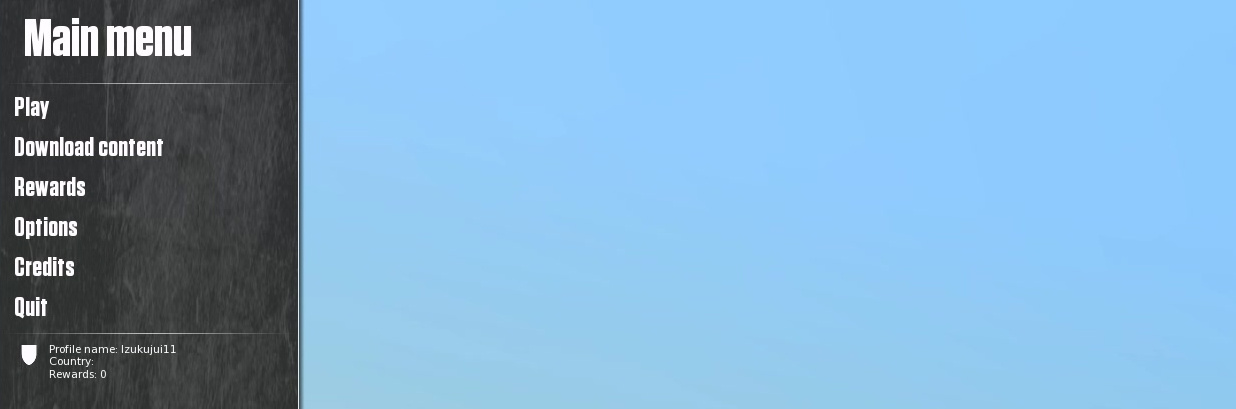
\includegraphics[width=0.7\columnwidth]{picture/Main menu}
				%\captionsetup{font=scriptsize}
				\caption{
					\label{fig: Main menu} 
					主菜单界面。
				}
			\end{figure}
			
			启动进入游戏界面,随后进入游戏主菜单,主菜单至少需要包含 \textbf{Play},\textbf{Options}, \textbf{Quit}, 可以包含 \textbf{Credits} 和 \textbf{Rewards}。
			
				\subsubsection{Play}
				
				\begin{figure}[htbp]
					% read manual to see what [ht] means and for other possible options
					\centering 
					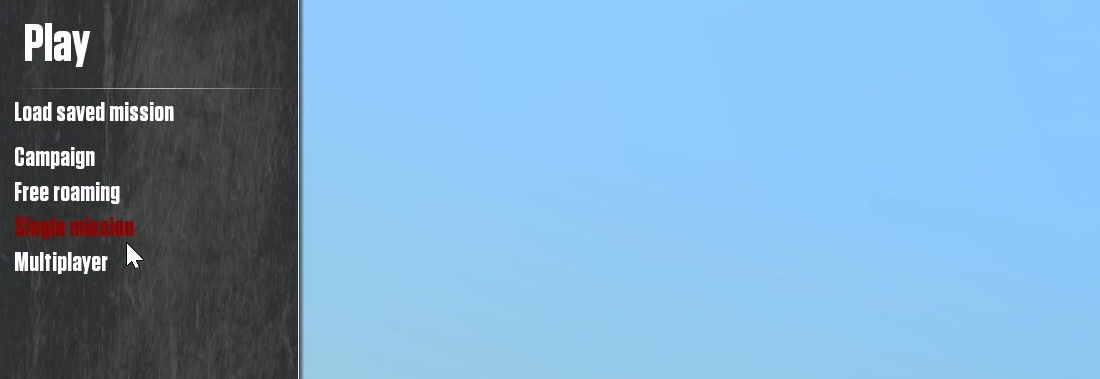
\includegraphics[width=0.7\columnwidth]{picture/Play}
					%\captionsetup{font=scriptsize}
					\caption{
						\label{fig: Play} 
						\textbf{Play} 菜单界面。
					}
				\end{figure}
				
				通过射线选择 \textbf{Play} 进入 \textbf{Play} 菜单,\textbf{Play} 菜单至少需要包含 \textbf{Free roaming}, 可以包含 \textbf{Campaign}, \textbf{Single mission}, \textbf{Load saved mission}。玩家通过射线,选择不同的选项进入不同的游戏模式。
				
				\paragraph{Free roaming} 
				
				\textbf{Free roaming} 游戏模式赋予玩家极大的游戏自由度,进入该模式之后,玩家可以选择不同的船只与地图,同时自定义不同的海况;
				
				\paragraph{Campaign}
				
				-
				
				\paragraph{Single mission}
				
				-
				
				\paragraph{Multiplayer}
				
				-
				
				\paragraph{Load saved mission}
				
				-
				
				\subsubsection{Options}
				
					\paragraph{Controls}
					
					\begin{figure}[htbp]
						% read manual to see what [ht] means and for other possible options
						\centering 
						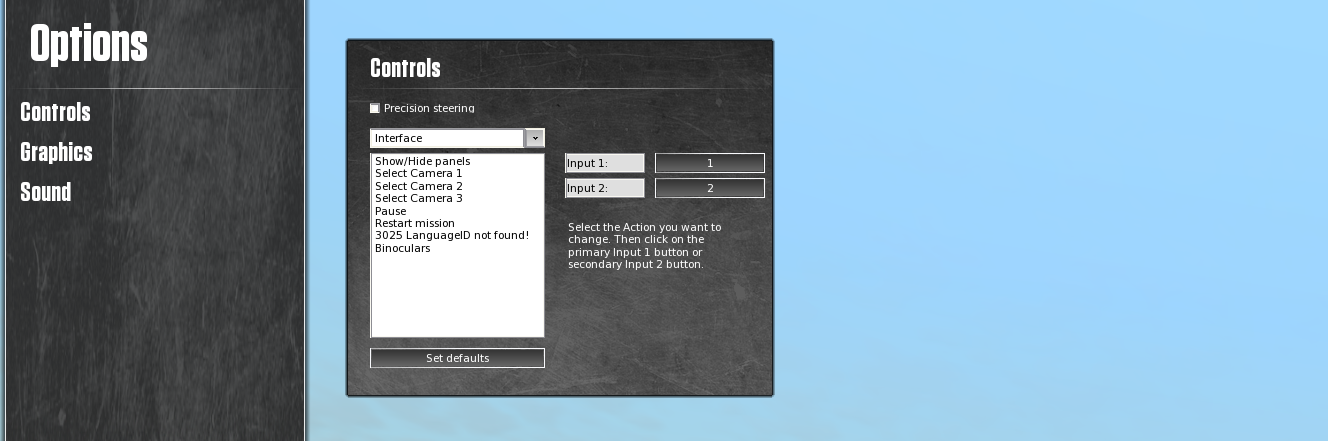
\includegraphics[width=0.7\columnwidth]{picture/Options_Controls}
						%\captionsetup{font=scriptsize}
						\caption{
							\label{fig: Options_Controls} 
							\textbf{Controls} 选项界面。
						}	
					\end{figure}
					
					\textbf{Controls} 可以设置不同的控制模式,一种是对船面板的控制(第一人称视角),如Fig. \ref{fig: First-person perspective}所示。;另一种是以(第三人称视角)对船进行控制,并实现多种不同的第三人称视角,即多个 Camera ;最后是可以对船的控制进行自定义控制,如引擎推动开关和方向控制键。
					
					\begin{figure}[htbp]
						% read manual to see what [ht] means and for other possible options
						\centering
						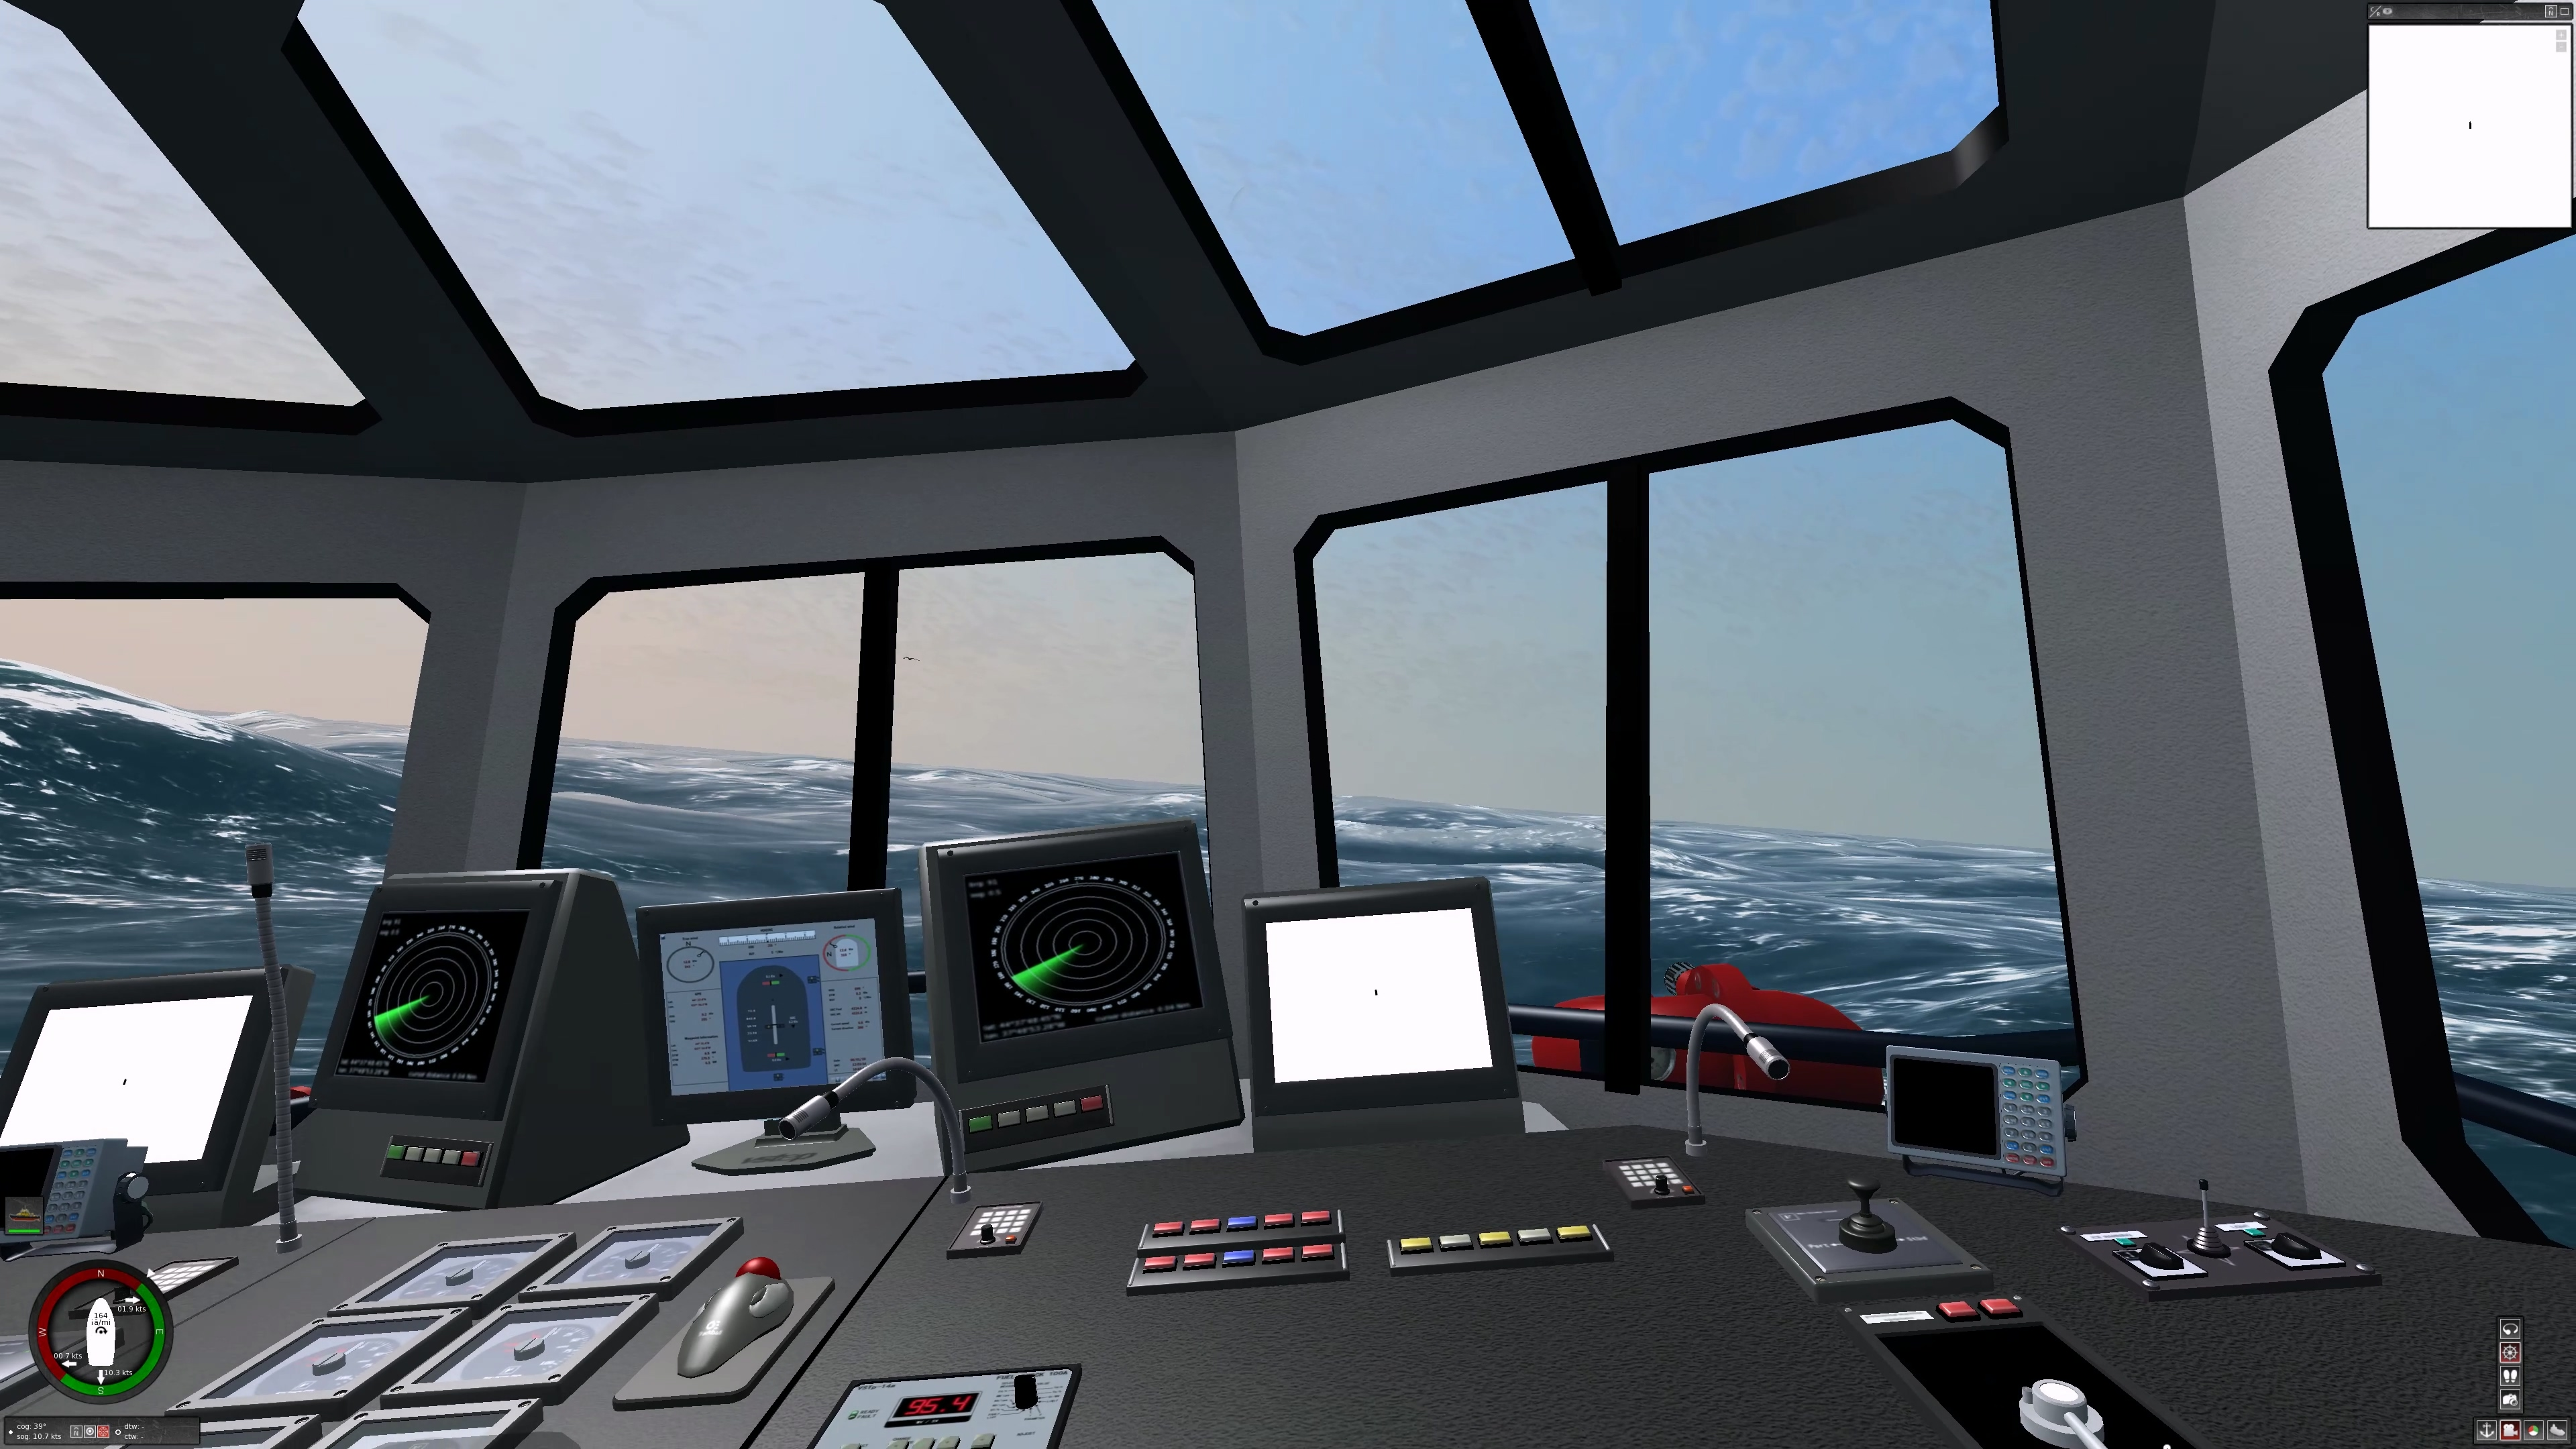
\includegraphics[width=\columnwidth]{picture/First-person perspective}
						%\captionsetup{font=scriptsize}
						\caption{
							\label{fig: First-person perspective} 
							第一人称视角游玩。
						}	
					\end{figure}
					
					
					\paragraph{Graphics}
					
					\begin{figure}[htbp]
						% read manual to see what [ht] means and for other possible options
						\centering 
						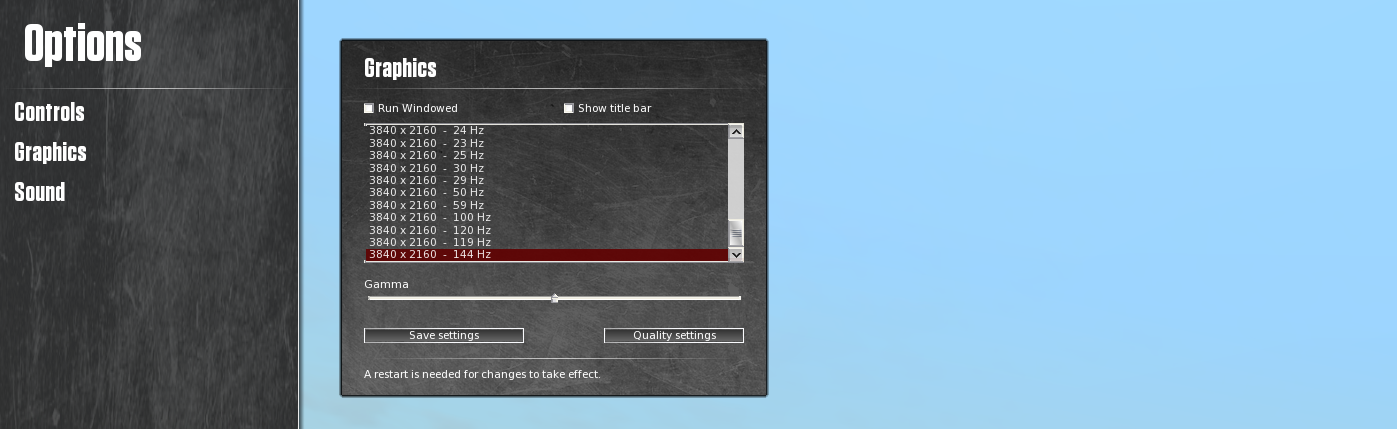
\includegraphics[width=0.7\columnwidth]{picture/Options_Graphics}
						%\captionsetup{font=scriptsize}
						\caption{
							\label{fig: Options_Graphics} 
							\textbf{Graphics} 选项界面。
						}	
					\end{figure}
					
					\textbf{Graphics} 可以设置分辨率、是否窗口模式运行、设置刷新率和游戏渲染质量,并能够生成相应的保存的文件,每次启动时读取该保存文件。
					
					\paragraph{Sound}
					
					\begin{figure}[htbp]
						% read manual to see what [ht] means and for other possible options
						\centering 
						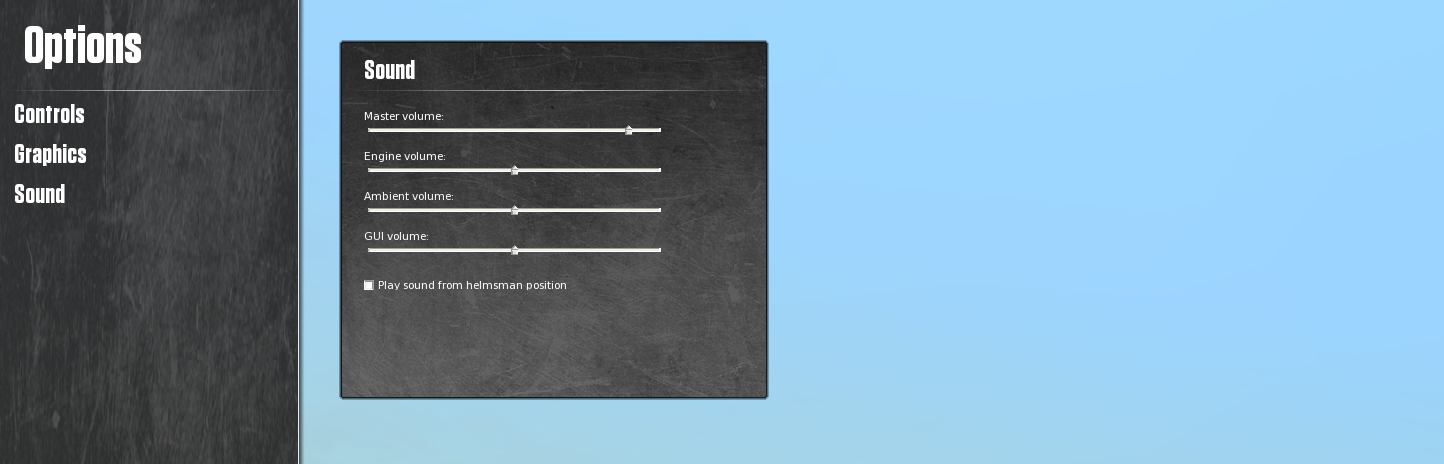
\includegraphics[width=0.7\columnwidth]{picture/Options_Sound}
						%\captionsetup{font=scriptsize}
						\caption{
							\label{fig: Options_Sound} 
							\textbf{Sound} 选项界面。
						}	
					\end{figure}
					
					\textbf{Sound} 可以设置总音量(Master volume)、船只引擎的音量(Engine volume)、环境音乐的音量(Ambient volume)、界面音量( GUI volume)
				
				\subsubsection{Quit}
				
				退出游戏,即终止游戏程序运行。
				
				\subsubsection{Credits}
				
				游戏信息的展示,在主界面的滚动显示,或者是弹窗显示均可。
				
				\subsubsection{Rewards}
	
				游戏的奖杯模式,需要建立相应的任务系统,完成相应的任务之后跳杯,获得的奖杯可以在此处显示。
	
			\subsection{游戏模式}
	
				\subsubsection{Free roaming}
				
				\paragraph{船只模型自定义}
				
				\begin{figure}[htbp]
					% read manual to see what [ht] means and for other possible options
					\centering 
					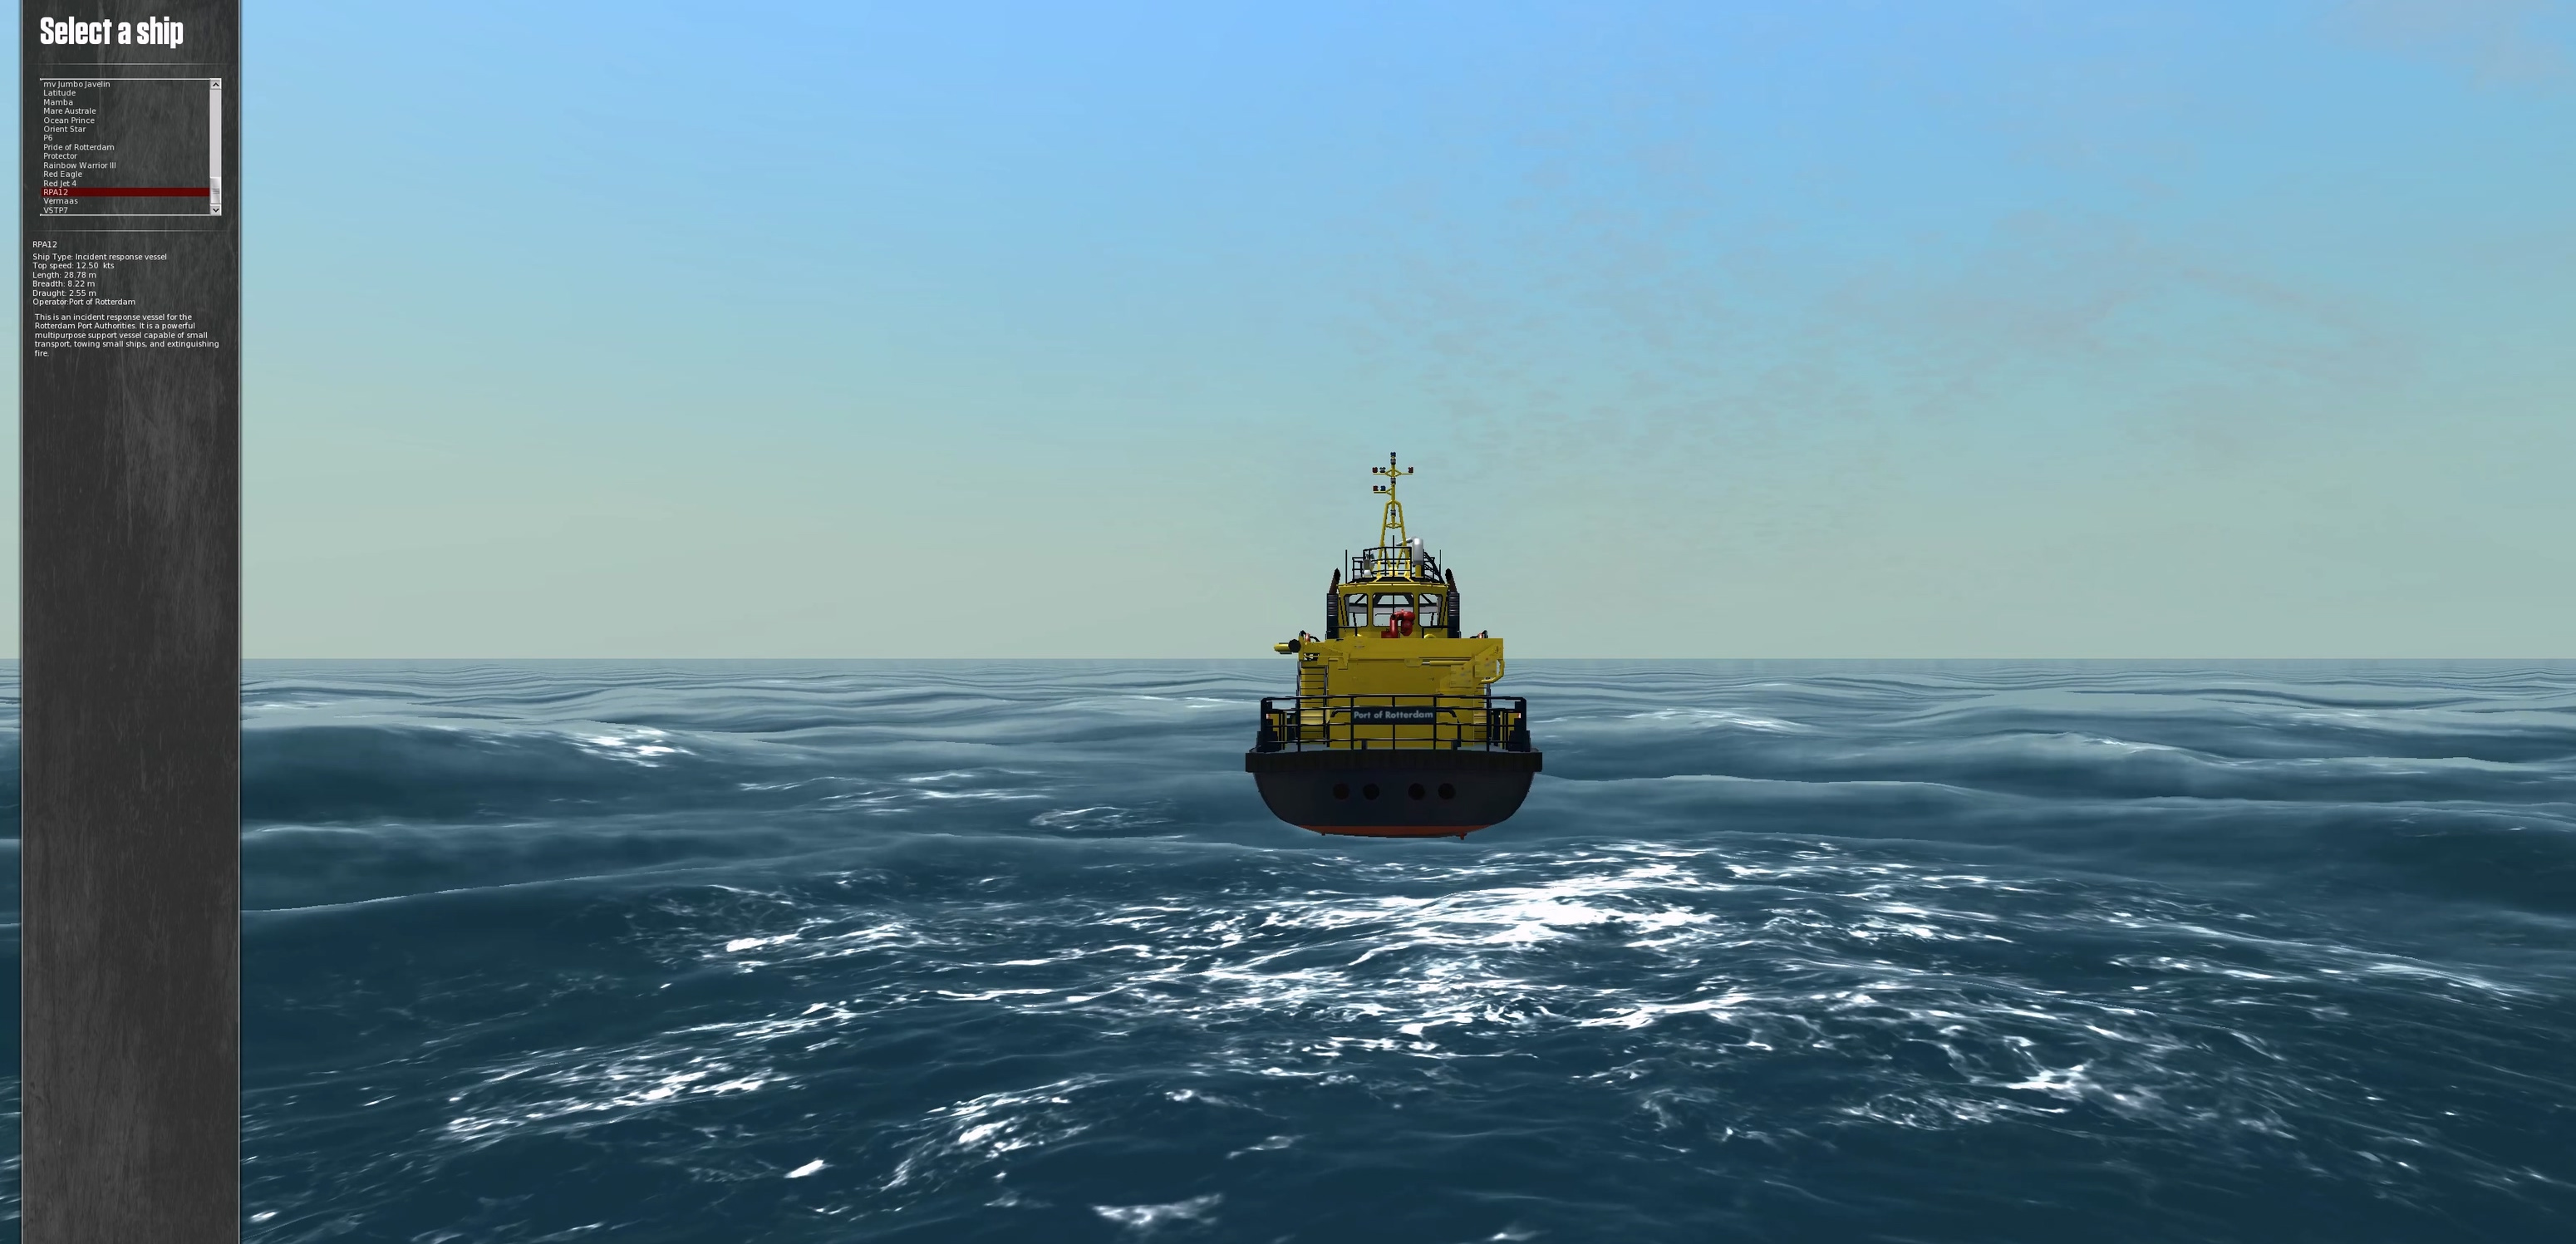
\includegraphics[width=0.7\columnwidth]{picture/Select a ship}
					%\captionsetup{font=scriptsize}
					\caption{
						\label{fig: Select a ship} 
						船只模型选择界面。
					}	
				\end{figure}
	
				\textbf{Free roaming}下玩家可以任意进行船只选择,不同的船只会有不同的参数,如转向半径、平稳程度、马力、船只大小等会有明显区别。并且进行选择时,该船只会出现在主界面上,玩家可以直观的看到所选择的船只模型。
				
				\paragraph{环境自定义}
				
				\begin{figure}[htbp] 
					% read manual to see what [ht] means and for other possible options
					\centering 
					% 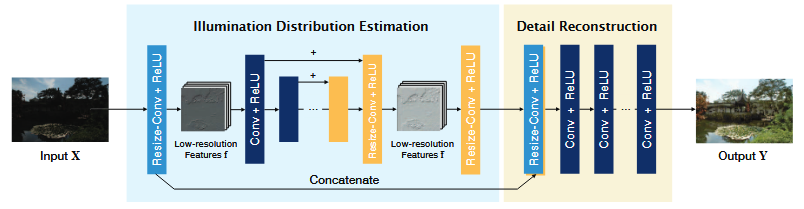
\includegraphics[width=0.8\columnwidth]{GLADNet}
					
					\begin{subfigure}{0.24\textwidth}
						\includegraphics[width=\linewidth]{picture/Environment_Antarctic}
						\captionsetup{font=scriptsize}
						\caption{Antarctic}
						\label{fig: Environment_Antarctic}
					\end{subfigure}
					\begin{subfigure}{0.24\textwidth}
						\includegraphics[width=\linewidth]{picture/Environment_Atlantic Ocean}
						\captionsetup{font=scriptsize}
						\caption{Atlantic Ocean}
						\label{fig: Environment_Atlantic Ocean}
					\end{subfigure}
					\begin{subfigure}{0.24\textwidth}
						\includegraphics[width=\linewidth]{picture/Environment_Bora Bora}
						\captionsetup{font=scriptsize}
						\caption{Bora Bora}
						\label{fig: Environment_Bora Bora}	
					\end{subfigure}
					\begin{subfigure}{0.24\textwidth}
						\includegraphics[width=\linewidth]{picture/Environment_Dover}
						\captionsetup{font=scriptsize}
						\caption{Dover}
						\label{fig: Environment_Dover}	
					\end{subfigure} \\

					\begin{subfigure}{0.24\textwidth}
						\includegraphics[width=\linewidth]{picture/Environment_Hamburg}
						\captionsetup{font=scriptsize}
						\caption{Hamburg}
						\label{fig: Environment_Hamburg}
					\end{subfigure}
					\begin{subfigure}{0.24\textwidth}
						\includegraphics[width=\linewidth]{picture/Environment_Marseille}
						\captionsetup{font=scriptsize}
						\caption{Marseille}
						\label{fig: Environment_Marseille}
					\end{subfigure}
					\begin{subfigure}{0.24\textwidth}
						\includegraphics[width=\linewidth]{picture/Environment_New York}
						\captionsetup{font=scriptsize}
						\caption{New York}
						\label{fig: Environment_New York}	
					\end{subfigure}
					\begin{subfigure}{0.24\textwidth}
						\includegraphics[width=\linewidth]{picture/Environment_Padstow, Cornwall}
						\captionsetup{font=scriptsize}
						\caption{Padstow, Cornwall}
						\label{fig: Environment_Padstow, Cornwall}	
					\end{subfigure} \\

					\begin{subfigure}{0.24\textwidth}
						\includegraphics[width=\linewidth]{picture/Environment_Port of Rotterdam}
						\captionsetup{font=scriptsize}
						\caption{Port of Rotterdam}
						\label{fig: Environment_Port of Rotterdam}
					\end{subfigure}
					\begin{subfigure}{0.24\textwidth}
						\includegraphics[width=\linewidth]{picture/Environment_San Francisco}
						\captionsetup{font=scriptsize}
						\caption{San Francisco}
						\label{fig: Environment_San Francisco}
					\end{subfigure}
					\begin{subfigure}{0.24\textwidth}
						\includegraphics[width=\linewidth]{picture/Environment_Sydney}
						\captionsetup{font=scriptsize}
						\caption{Sydney}
						\label{fig: Environment_Sydney}	
					\end{subfigure}
					\begin{subfigure}{0.24\textwidth}
						\includegraphics[width=\linewidth]{picture/Environment_The Solent}
						\captionsetup{font=scriptsize}
						\caption{The Solent}
						\label{fig: Environment_The Solent}	
					\end{subfigure}
					
					\captionsetup{font=scriptsize}
					\caption{
						\label{fig: Environment selection}
						在 \textbf{Free roaming} 下,玩家可以在Environment界面中自定义来自世界各地的海面环境。
					}
				\end{figure}
				
				此外,在不同的地图场景下,可以自定义船只起始出发的地点。如Fig. \ref{fig: Starting point selection}所示,在 New York 港口一共可以选择9个出发点,开始自由航行。
				
				\begin{figure}[htbp]
					% read manual to see what [ht] means and for other possible options
					\centering 
					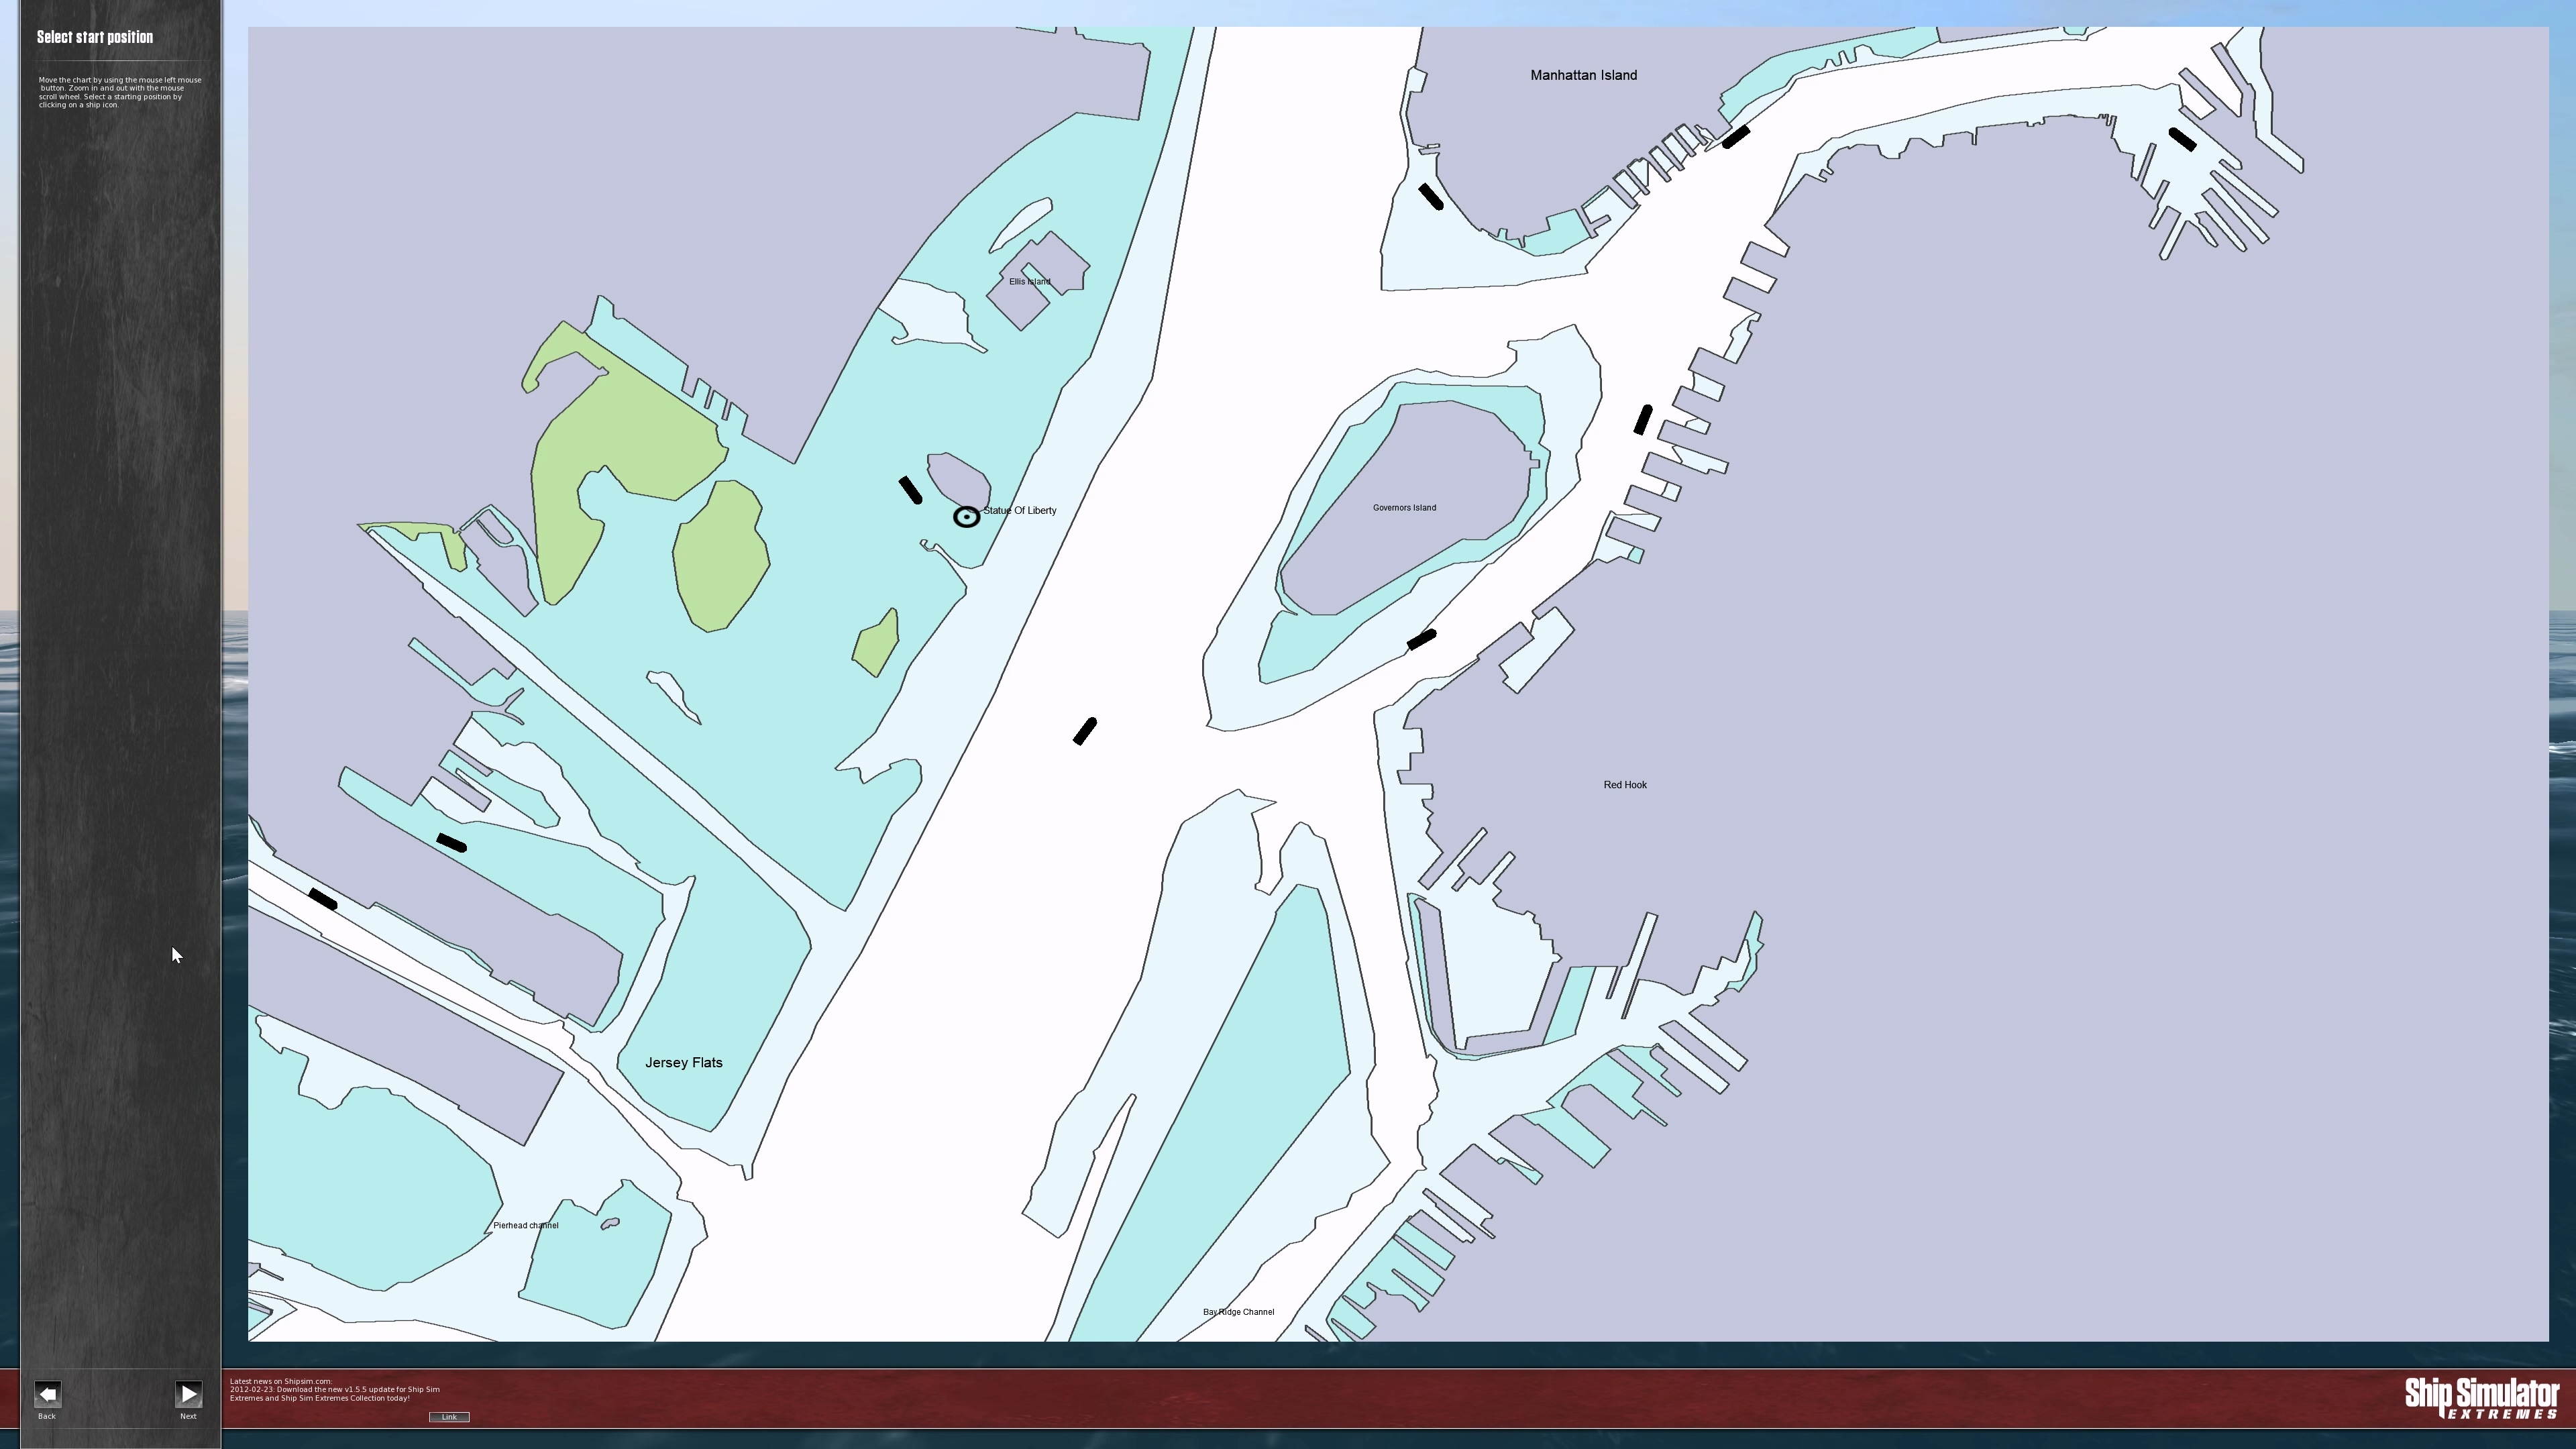
\includegraphics[width=0.7\columnwidth]{picture/Starting point selection}
					%\captionsetup{font=scriptsize}
					\caption{
						\label{fig: Starting point selection} 
						在纽约港口环境下,船只出发地点选择。
					}	
				\end{figure}
				
				\paragraph{天气自定义}
				
				\begin{figure}[htbp]
					% read manual to see what [ht] means and for other possible options
					\centering 
					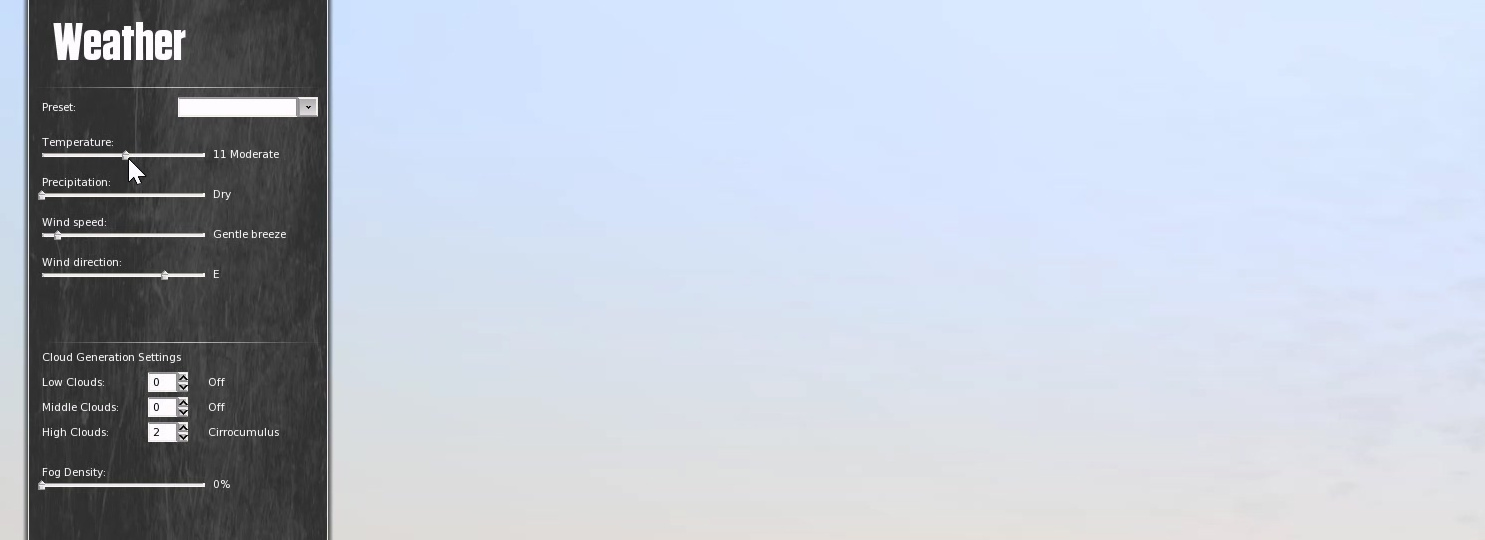
\includegraphics[width=0.7\columnwidth]{picture/Weather}
					%\captionsetup{font=scriptsize}
					\caption{
						\label{fig: Weather} 
						天气自定义界面。
					}	
				\end{figure}
				
				\textbf{Free roaming}下玩家也可以自定义各类海洋天气,以实现不同海况下的航行。可以设置不同的 \textbf{Temperature}、\textbf{Precipitation}、 \textbf{Wind speed}、 \textbf{Wind direction} 等参数,来实现不同的海况。
				
				
				主要参数有6种,每一种的定义如下:
				\begin{itemize}
					\item [(1)] 
					\textbf{Temperature} 设置4个类别,共60个等级,其中 Freezing $[-20 \sim -1]$、Cold $[0 \sim 9]$、Moderate $[10 \sim 19]$、Warm $[20 \sim 29]$、Hot $[30 \sim 40]$,单位为摄氏度。
					
					\item [(2)]
					\textbf{Precipitation} 设置5个等级,其中分别为 Dry, Drizzle, Rain, Heavy Rain, Cloudburst。
					
					\item [(3)]
					\textbf{Wind speed} 设置13个等级,其中分别为 Calm, Light air, Light breeze, Gentle breeze, Moderate breeze, Fresh breeze, Strong breeze, Moderate gale, Fresh gale, Strong gale, Storm, Violent Storm, Hurricane。
					
					\item [(4)]
					\textbf{Wind direction} 设置16个等级,其中分别为 S, SSW, SW, WSW, W, WNW, NW, NNW, N, NNE, NE, ENE, E, ESE, SE, SSE, S。
					
					\item [(5)]
					\textbf{Cloud Generation Settings} 设置3个类别,分别设置 Low Clouds, Middle Clouds, High Clouds;Low Clouds 的又分为3类,其中为 0 off, 1 Nimbostratus(乱层云) 2 Cumulonimbus(积雨云); Middle Clouds 分为3类,其中为 0 off, 1 Altostratus(高层云), 2 Altocumulus(高积云); High Clouds 分为3类,其中 0 off, 1 Cirrus(卷云), 2 Cirrocumulus(卷积云)
					
					\item [(6)]
					\textbf{Fog Density} 则设置为 $0 \sim 100\%$,百分比越高,能见度越差。
				\end{itemize}
	
				玩家除了可以自定义天气以外,需要快捷的辅助玩家设置不同类型的天气,故引入 \textbf{Preset} 设定。\textbf{Preset} 设置了9种天气,每一种天气对应上述6种参数不同的设定。9种天气为 Clear sky, Drizzle(毛毛雨), Foggy, Hail(冰雹), Light snow, Rainy, Snow storm(暴风雪), Storm, Wind\footnote{在实际的开发中,只需要开发这9种对应的天气,如果对每一种参数搭配($60 \times 5 \times 13 \times 16 \times 9 \times 100$)都开发对应的天气,这样的话,开发成本会很大。}。
				
				\begin{figure}[htbp] 
					% read manual to see what [ht] means and for other possible options
					\centering 
					% 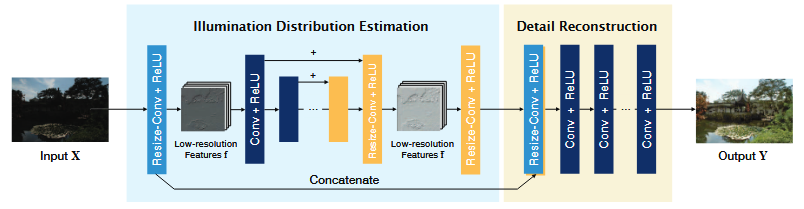
\includegraphics[width=0.8\columnwidth]{GLADNet}
					
					\begin{subfigure}{0.3\textwidth}
						\includegraphics[width=\linewidth]{picture/Clear sky}
						\captionsetup{font=scriptsize}
						\caption{Clear sky}
						\label{fig: Clear sky}
					\end{subfigure}
					\begin{subfigure}{0.3\textwidth}
						\includegraphics[width=\linewidth]{picture/Drizzle}
						\captionsetup{font=scriptsize}
						\caption{Drizzle}
						\label{fig: Drizzle}
					\end{subfigure}
					\begin{subfigure}{0.3\textwidth}
						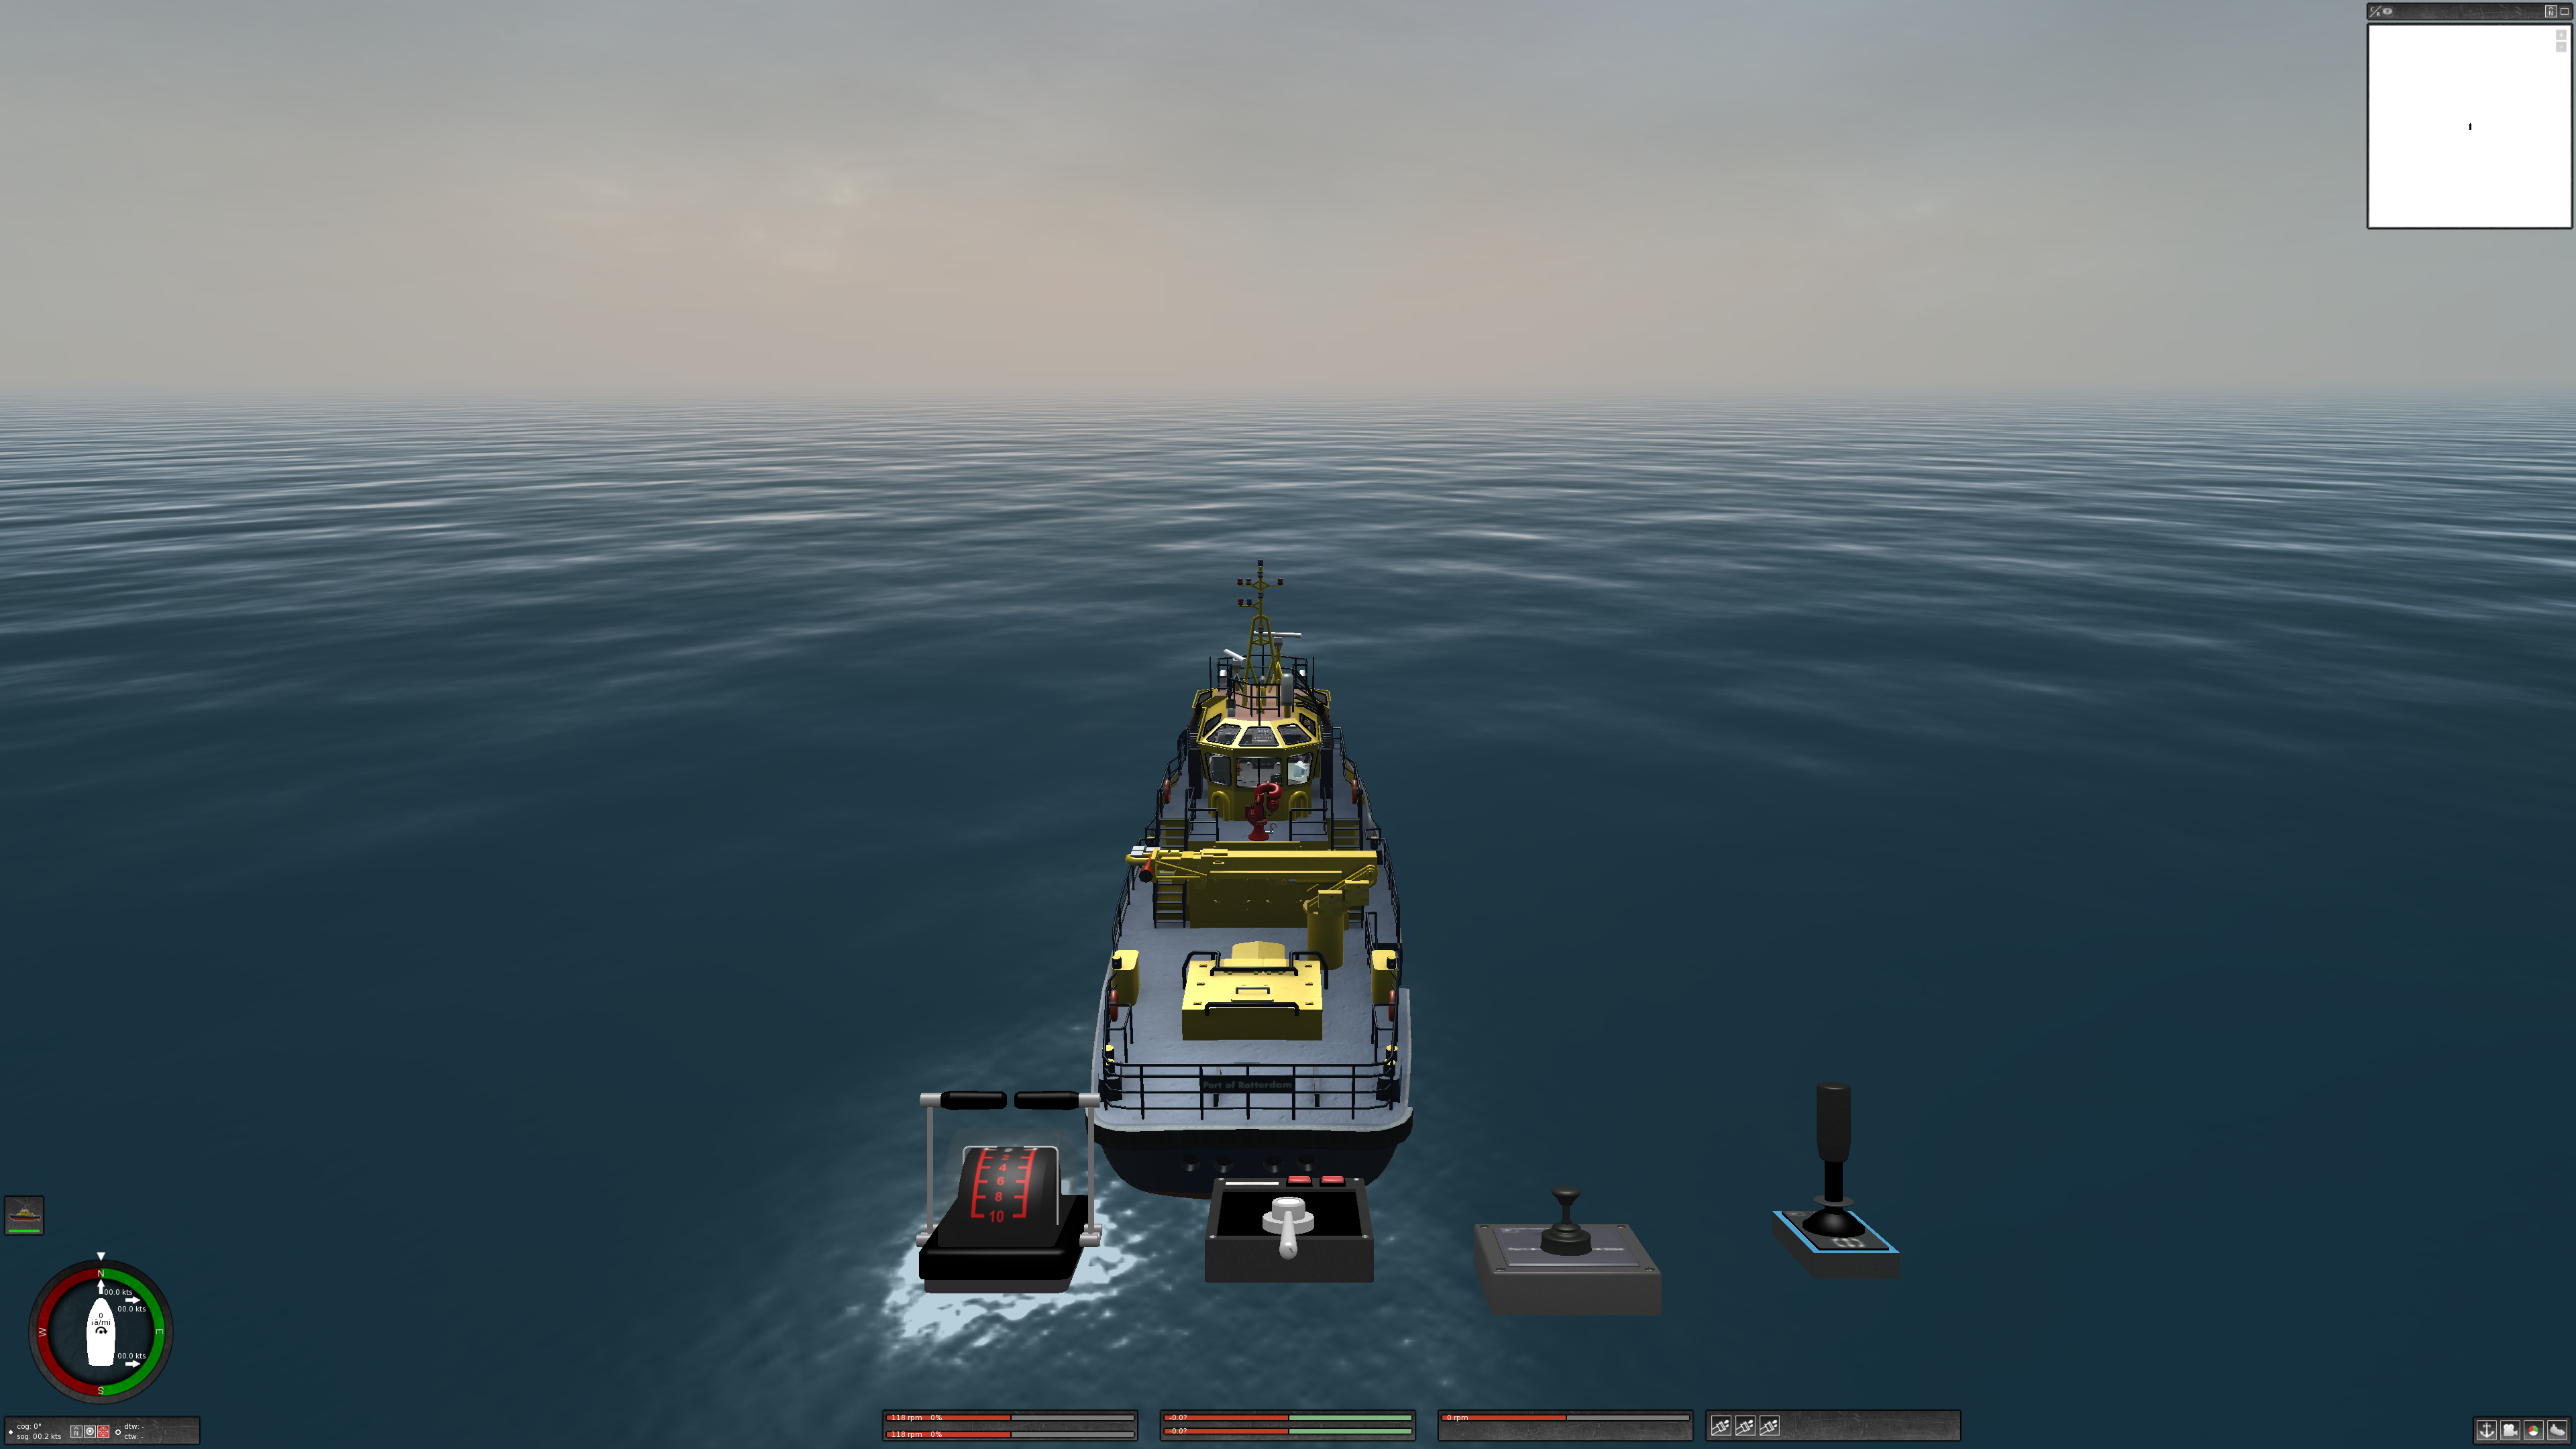
\includegraphics[width=\linewidth]{picture/Foggy}
						\captionsetup{font=scriptsize}
						\caption{Foggy}
						\label{fig: Foggy}	
					\end{subfigure}\\
					\begin{subfigure}{0.3\textwidth}
						\includegraphics[width=\linewidth]{picture/Hail}
						\captionsetup{font=scriptsize}
						\caption{Hail}
						\label{fig: Hail}	
					\end{subfigure}
					\begin{subfigure}{0.3\textwidth}
						\includegraphics[width=\linewidth]{picture/Light snow}
						\captionsetup{font=scriptsize}
						\caption{Light snow}
						\label{fig: Light snow}
					\end{subfigure}
					\begin{subfigure}{0.3\textwidth}
						\includegraphics[width=\linewidth]{picture/Rainy}
						\captionsetup{font=scriptsize}
						\caption{Rainy}
						\label{fig: Rainy}
					\end{subfigure}\\
					\begin{subfigure}{0.3\textwidth}
						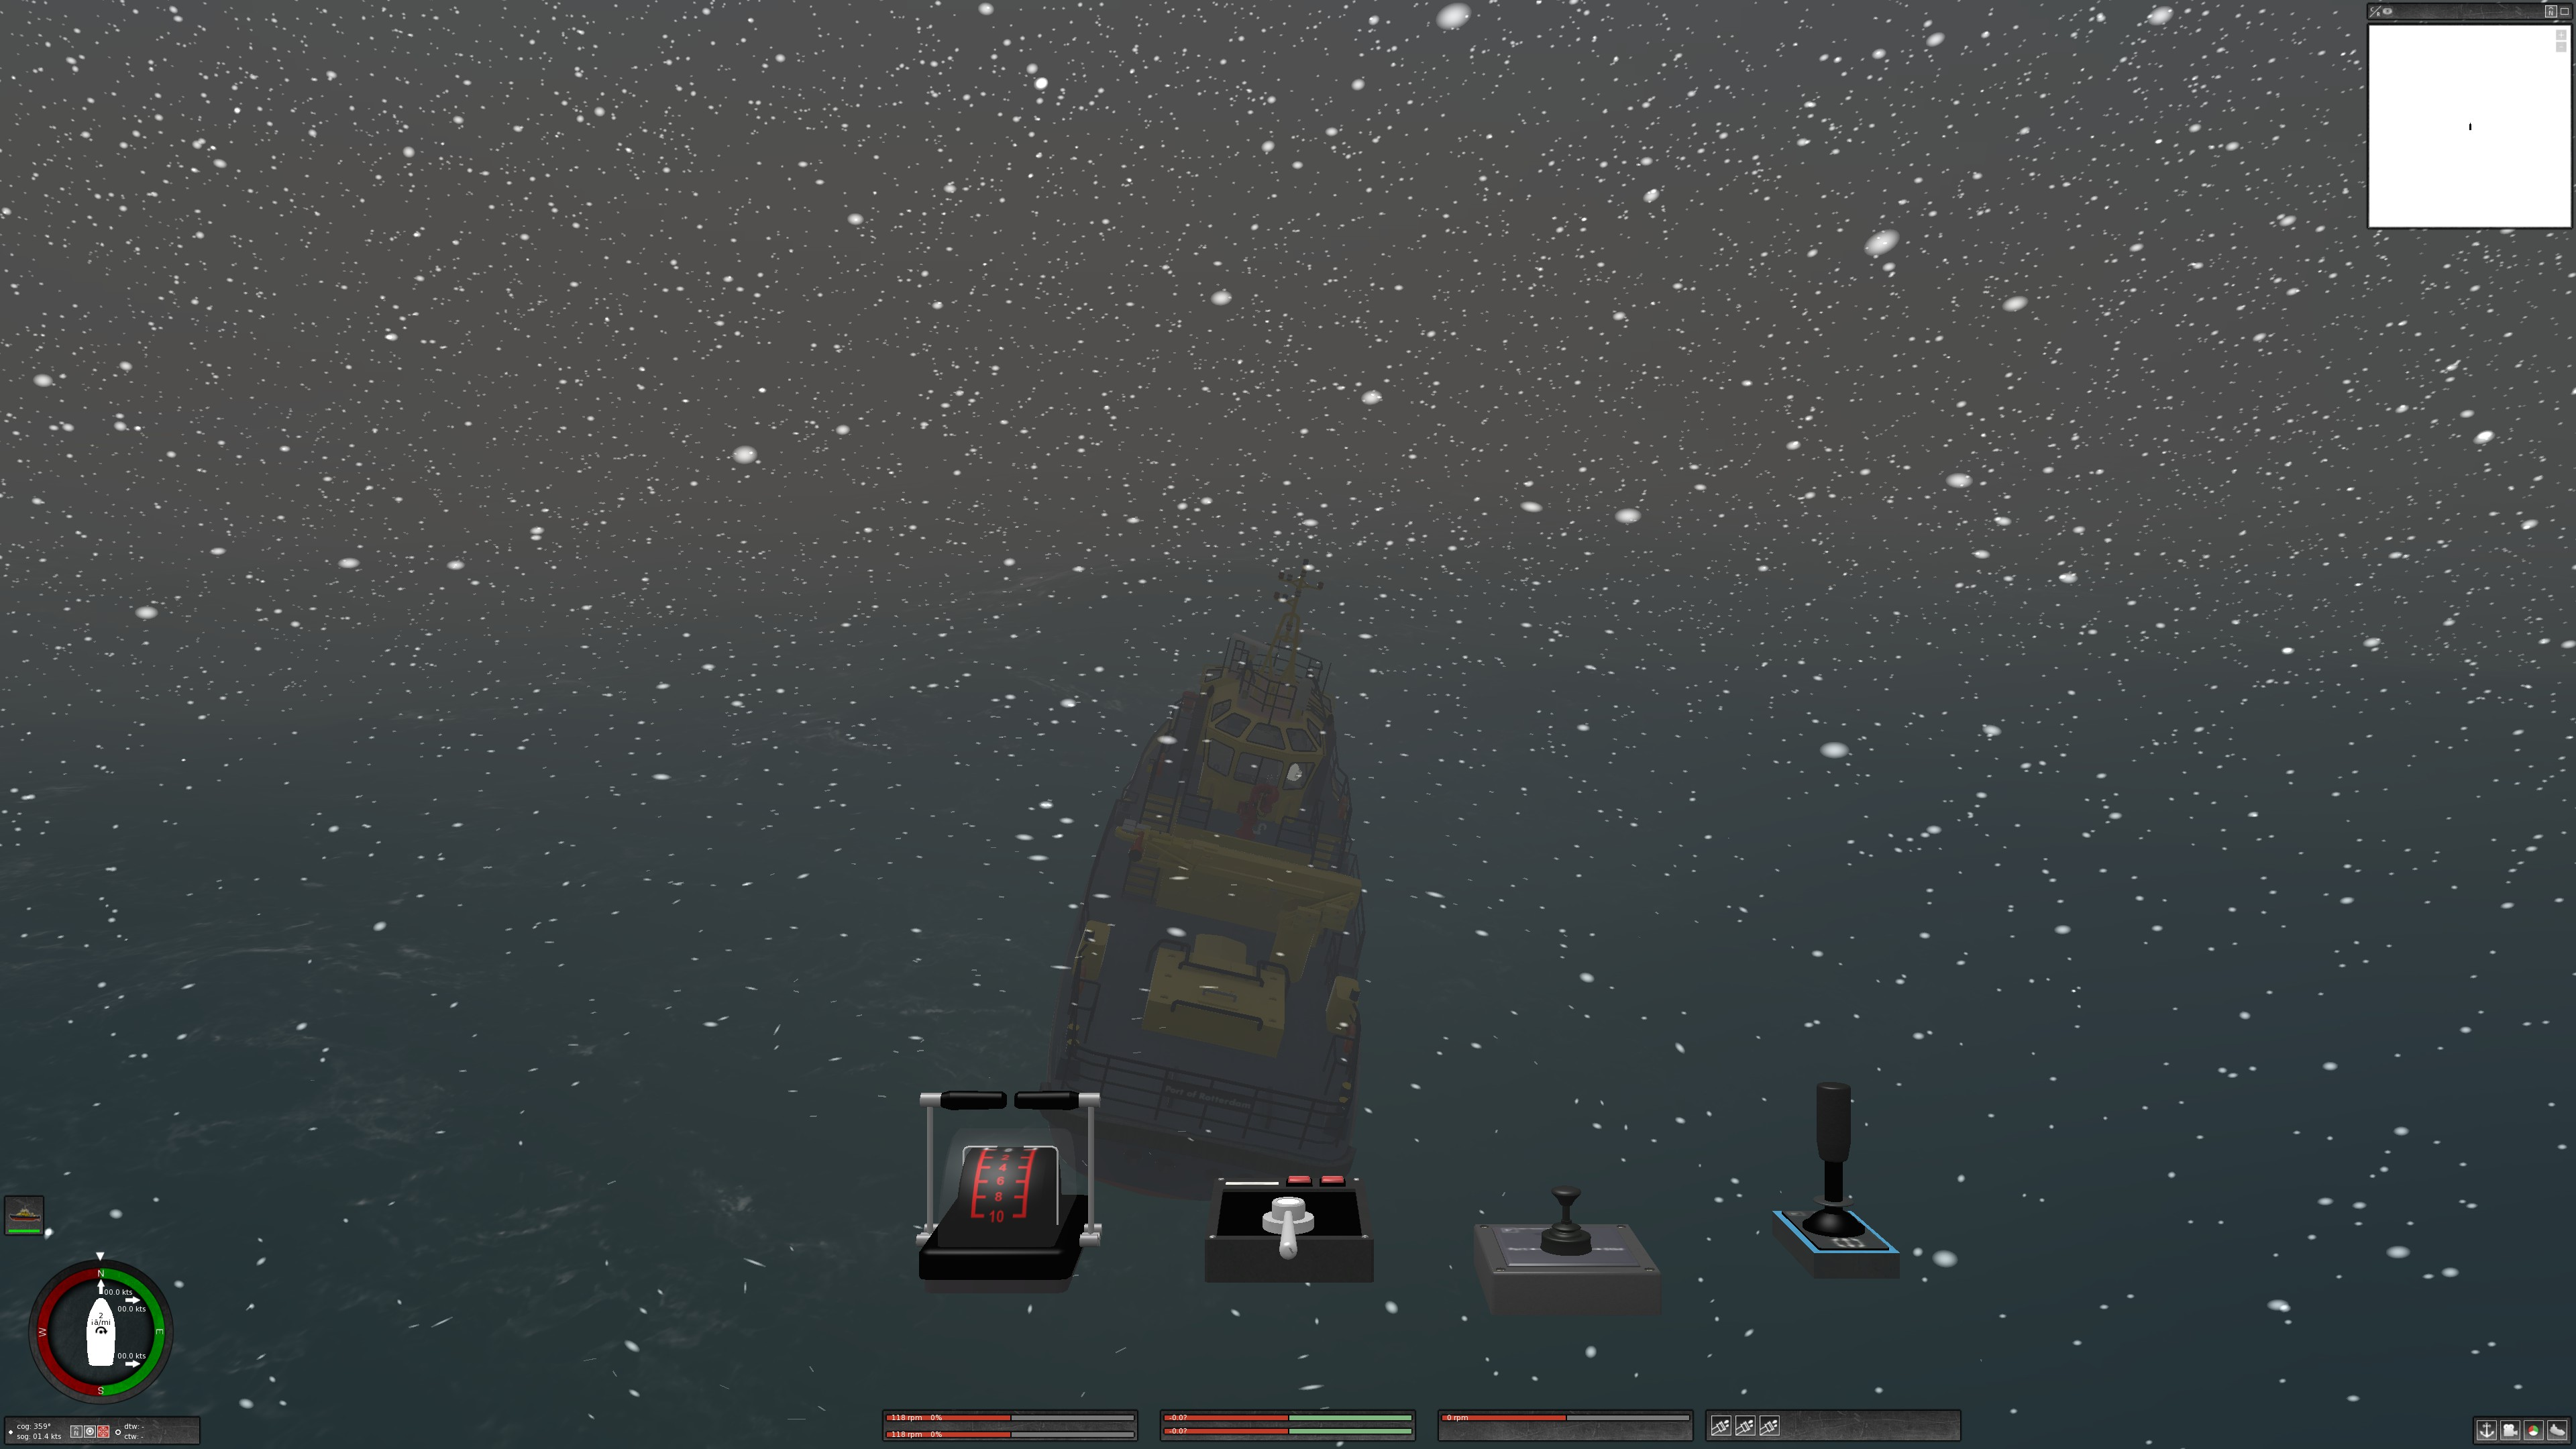
\includegraphics[width=\linewidth]{picture/Snow storm}
						\captionsetup{font=scriptsize}
						\caption{Snow storm}
						\label{fig: Snow storm}	
					\end{subfigure}
					\begin{subfigure}{0.3\textwidth}
						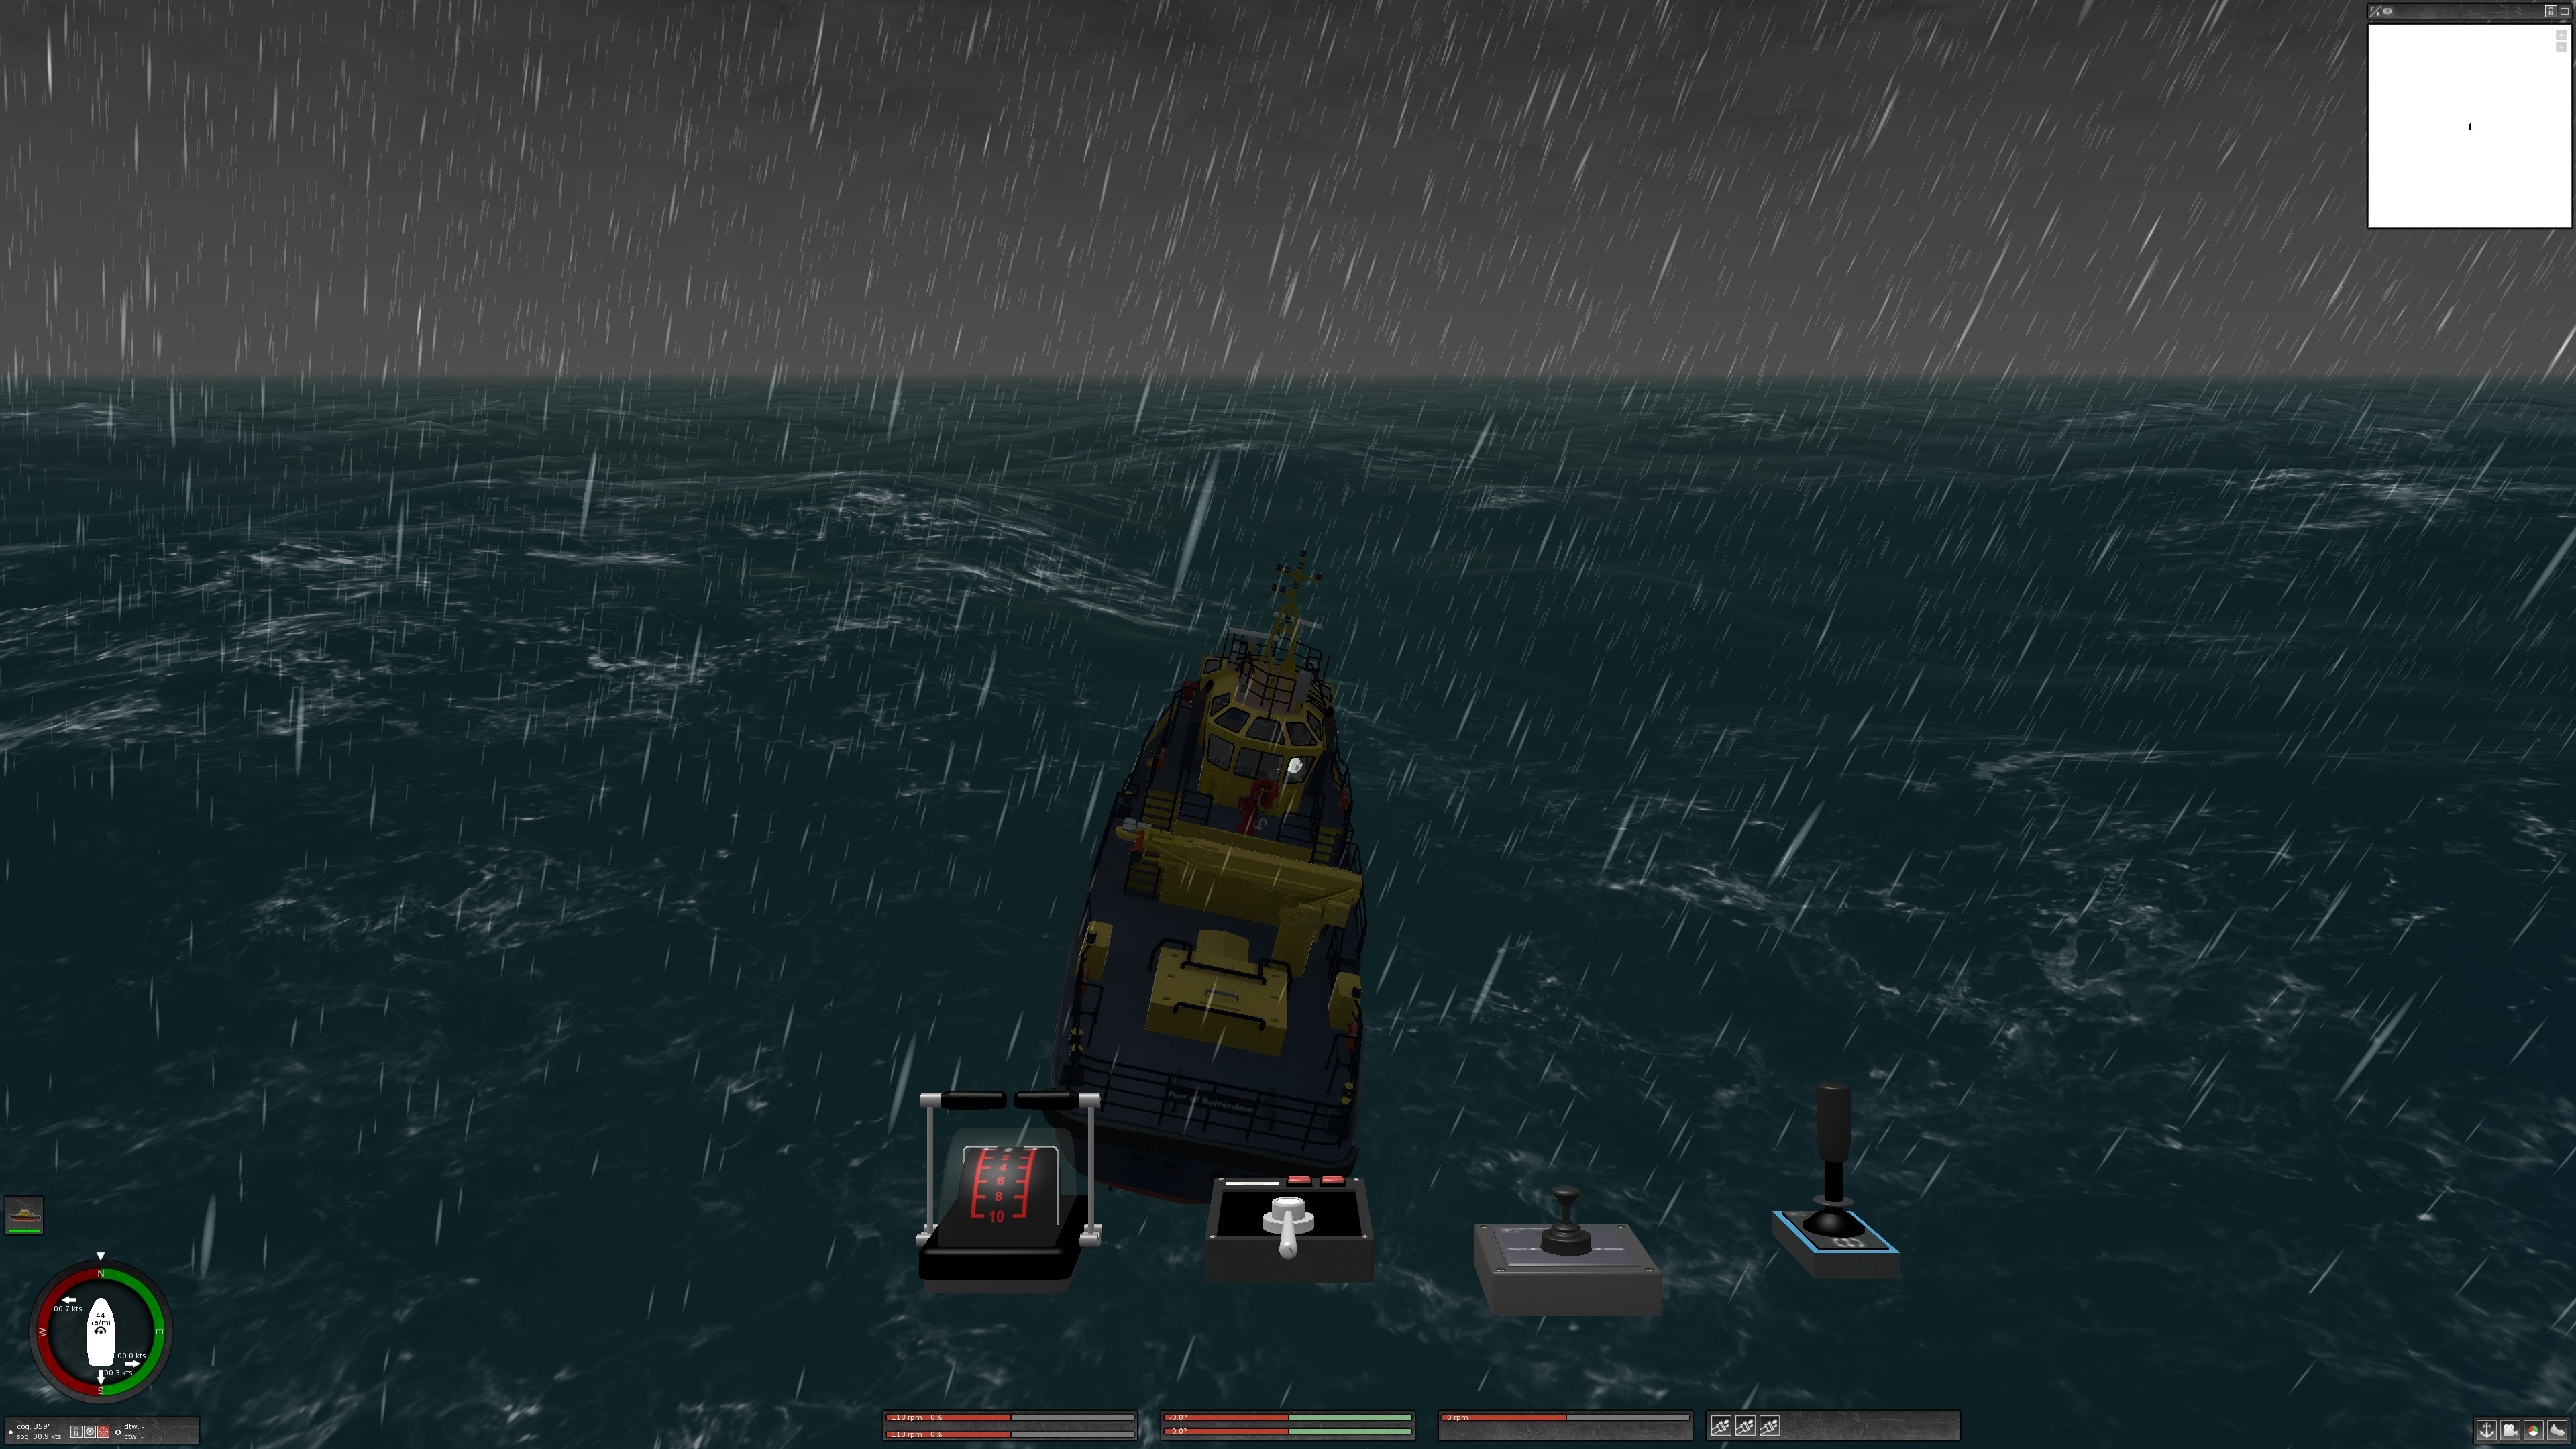
\includegraphics[width=\linewidth]{picture/Storm}
						\captionsetup{font=scriptsize}
						\caption{Storm}
						\label{fig: Storm}	
					\end{subfigure}
					\begin{subfigure}{0.3\textwidth}
						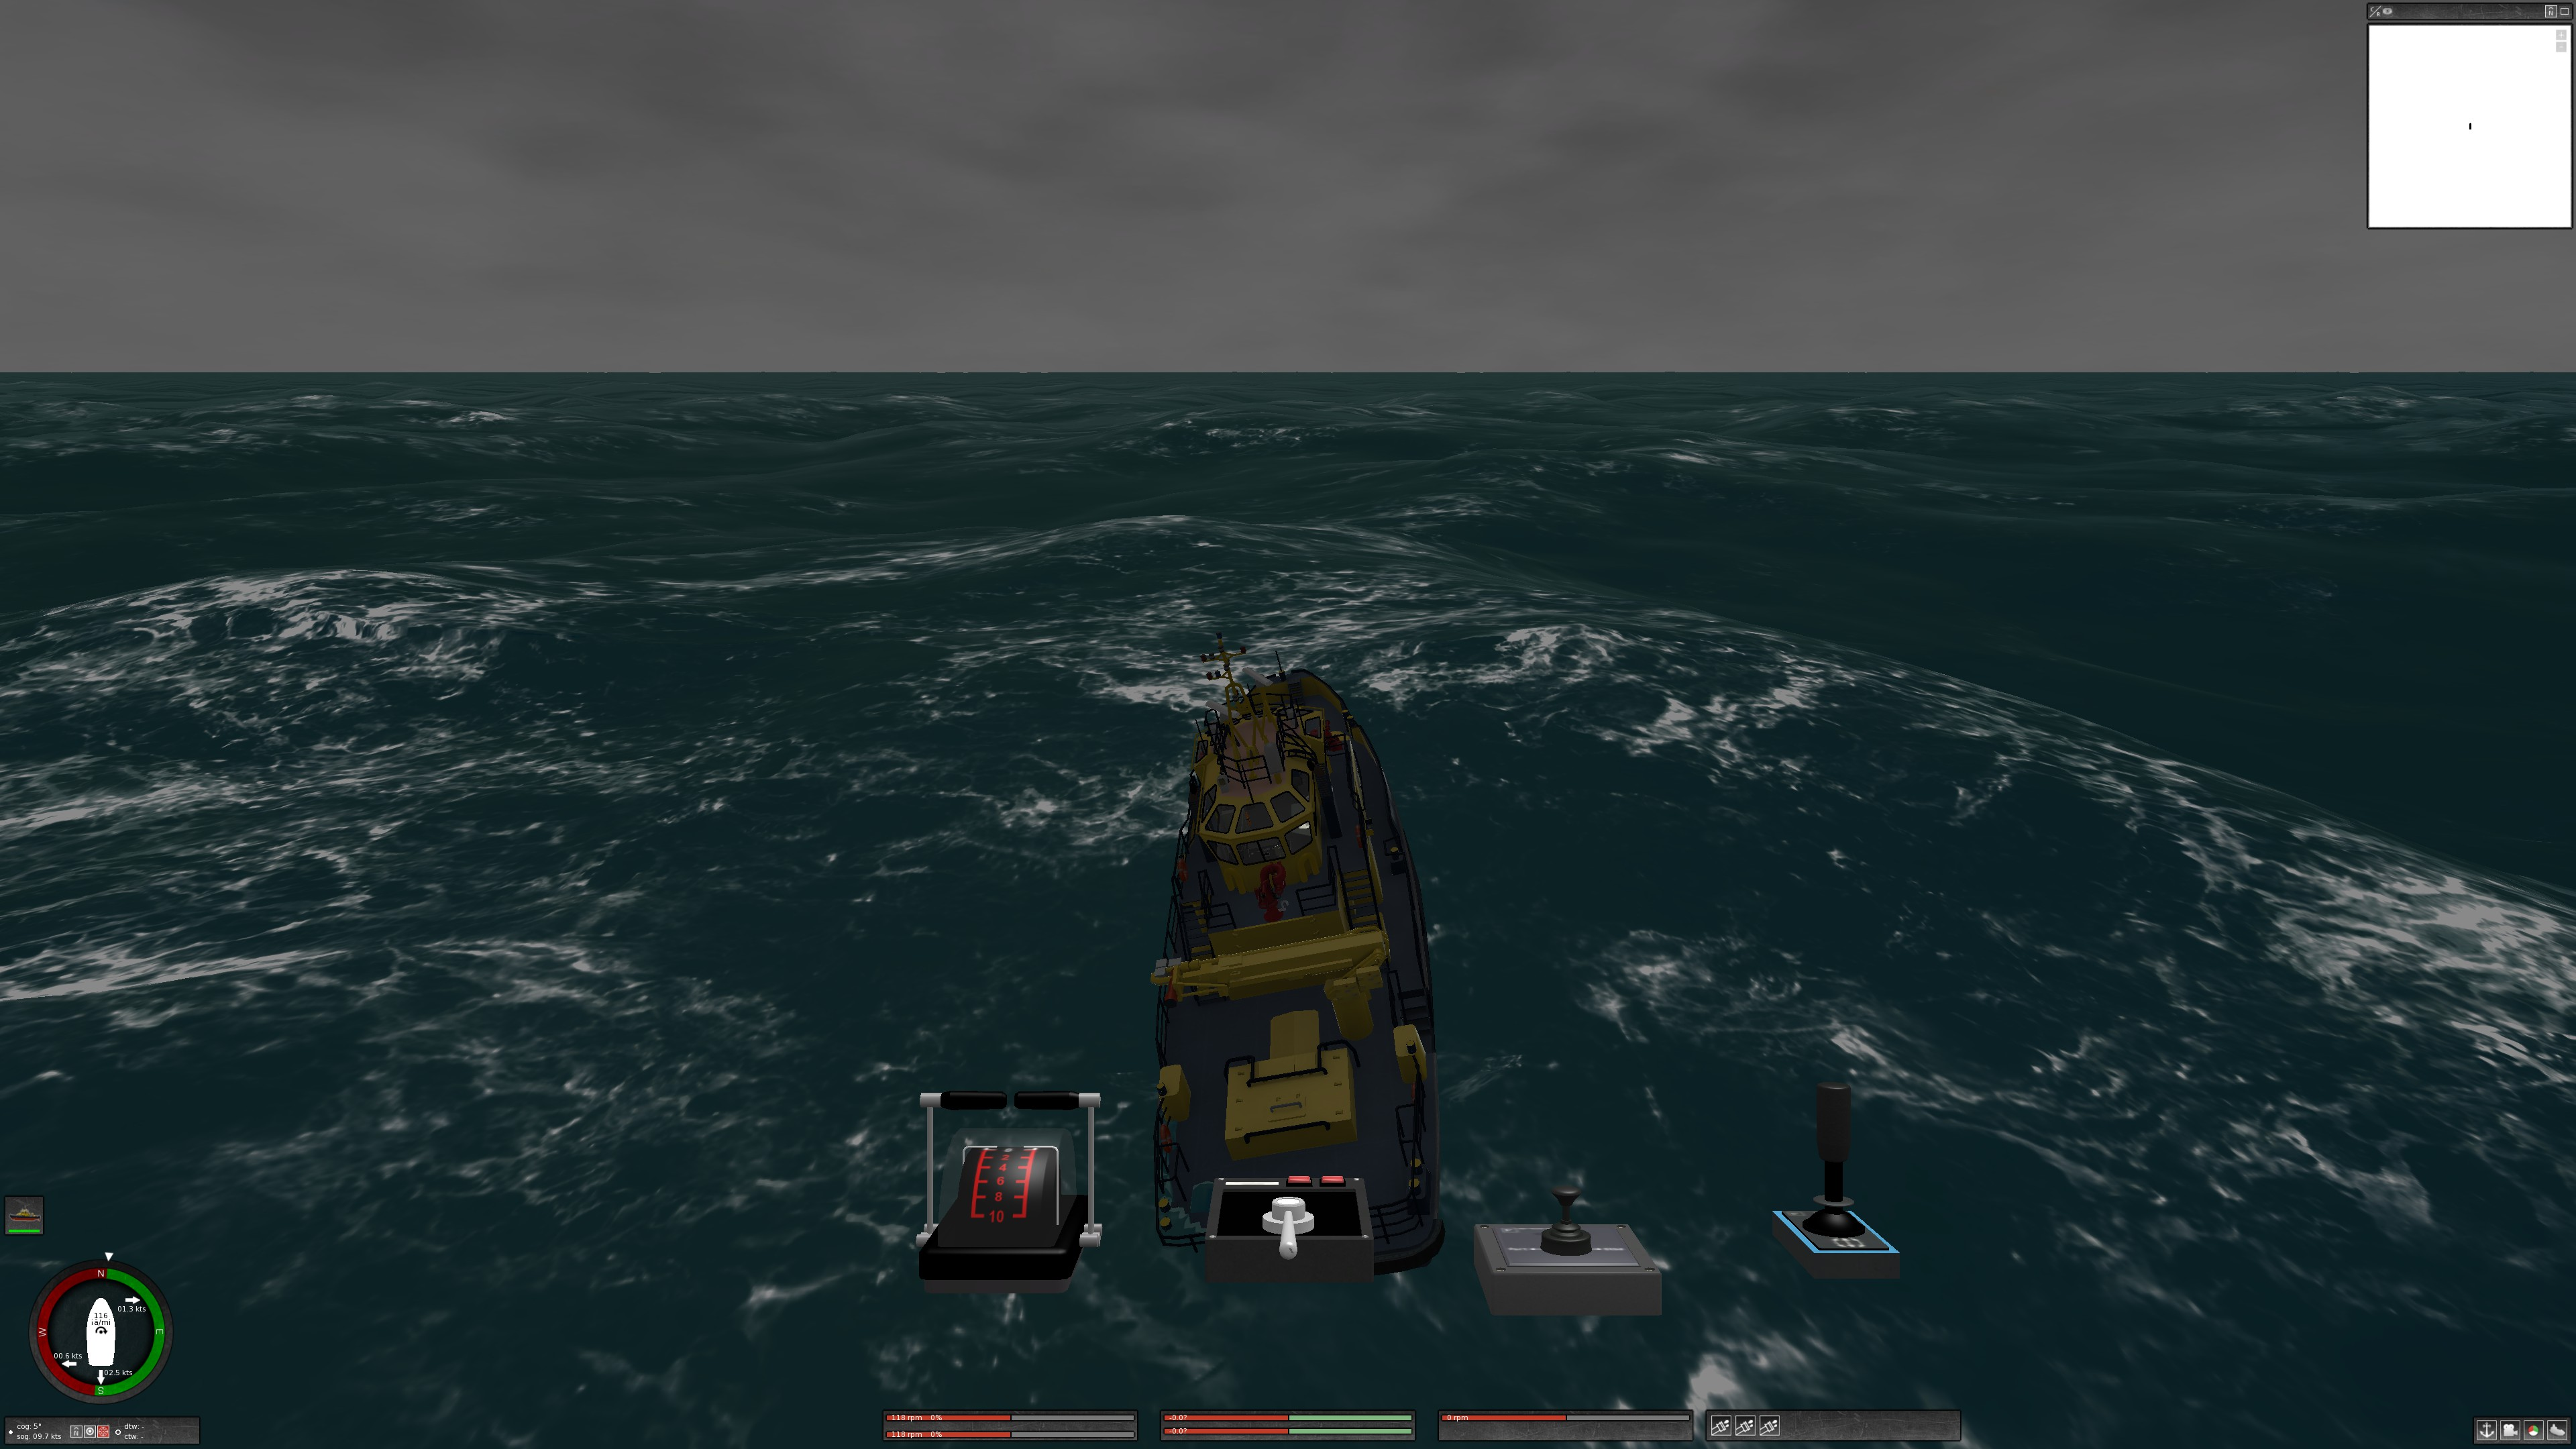
\includegraphics[width=\linewidth]{picture/Wind}
						\captionsetup{font=scriptsize}
						\caption{Wind}
						\label{fig: Wind}
					\end{subfigure}
					\captionsetup{font=scriptsize}
					\caption{
						\label{fig: Weather}
						9种不同的天气下的海况表现。
					}
				\end{figure}
			

	%	\section{Analysis}
	
	%	In this section you will need to show your experimental results. Use tables and
	%	graphs when it is possible. Table~\ref{tbl:bins} is an example.
	
	%	\begin{table}[ht]
		%		\begin{center}
			%			\caption{Every table needs a caption.}
			%			\label{tbl:bins} % spaces are big no-no withing labels
			%			\begin{tabular}{|ccc|} 
				%				\hline
				%				\multicolumn{1}{|c}{$x$ (m)} & \multicolumn{1}{c|}{$V$ (V)} & \multicolumn{1}{c|}{$V$ (V)} \\
				%				\hline
				%				0.0044151 &   0.0030871 &   0.0030871\\
				%				0.0021633 &   0.0021343 &   0.0030871\\
				%				0.0003600 &   0.0018642 &   0.0030871\\
				%				0.0023831 &   0.0013287 &   0.0030871\\
				%				\hline
				%			\end{tabular}
			%		\end{center}
		%	\end{table}
	%	
	%	Analysis of equation~\ref{eq:aperp} shows ...
	%	
	%	Note: this section can be integrated with the previous one as long as you
	%	address the issue. Here explain how you determine uncertainties for different
	%	measured values. Suppose that in the experiment you make a series of
	%	measurements of a resistance of the wire $R$ for different applied voltages
	%	$V$, then you calculate the temperature from the resistance using a known
	%	equation and make a plot  temperature vs. voltage squared. Again suppose that
	%	this dependence is expected to be linear~\cite{Cyr}, and the proportionality coefficient
	%	is extracted from the graph. Then what you need to explain is that for the
	%	resistance and the voltage the uncertainties are instrumental (since each
	%	measurements in done only once), and they are $\dots$. Then give an equation
	%	for calculating the uncertainty of the temperature from the resistance
	%	uncertainty. Finally explain how the uncertainty of the slop of the graph was
	%	found (computer fitting, graphical method, \emph{etc}.)
	%	
	%	If in the process of data analysis you found any noticeable systematic
	%	error(s), you have to explain them in this section of the report.
	%	
	%	It is also recommended to plot the data graphically to efficiently illustrate
	%	any points of discussion. For example, it is easy to conclude that the
	%	experiment and theory match each other rather well if you look at
	%	Fig.~\ref{fig:samplesetup} and Fig.~\ref{fig:exp_plots}.
	%	
	%	\begin{figure}[ht] 
		%		\centering
		%		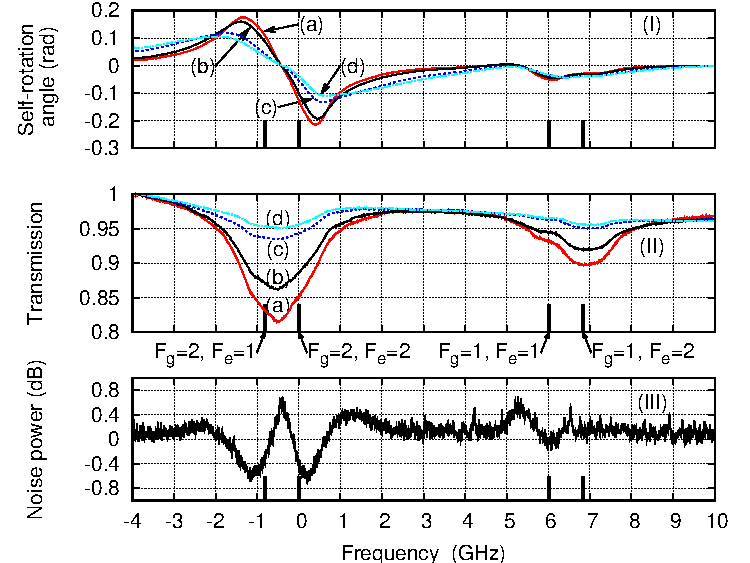
\includegraphics[width=0.5\columnwidth]{sr_squeezing_vs_detuning}
		%		
		%		% some figures do not need to be too wide
		%		\caption{
			%			\label{fig:exp_plots}  
			%			Every plot must have axes labeled.
			%		}
		%	\end{figure}
	
	
	%	\section{Conclusions}
	%	Here you briefly summarize your findings.
	
	%++++++++++++++++++++++++++++++++++++++++
	% References section will be created automatically 
	% with inclusion of "thebibliography" environment
	% as it shown below. See text starting with line
	% \begin{thebibliography}{99}
		% Note: with this approach it is YOUR responsibility to put them in order
		% of appearance.
		
		\renewcommand{\refname}{References}
		
		
		%	\begin{thebibliography}{00}
			
			%		\bibitem{b1}\label{cite:b1}
			%		W. Wang, C. Wei, W. Yang and J. Liu, "GLADNet: Low-Light Enhancement Network with Global Awareness," 2018 13th IEEE International Conference on Automatic Face \& Gesture Recognition (FG 2018), Xi'an, China, 2018, pp. 751-755, DOI: 10.1109/FG.2018.00118.
			
			%		\bibitem{b2}\label{cite:b2}
			%		A.\ Mahajan, K.\ Somaraj and M. Sameer, "Adopting Artificial Intelligence Powered ConvNet To Detect Epileptic Seizures," 2020 IEEE-EMBS Conference on Biomedical Engineering and Sciences (IECBES), Langkawi Island, Malaysia, 2021, pp. 427-432, DOI: 10.1109/IECBES48179.2021.9398832.
			
			%		\bibitem{Cyr}
			%		N.\ Cyr, M.\ T$\hat{e}$tu, and M.\ Breton,
			% "All-optical microwave frequency standard: a proposal,"
			%		IEEE Trans.\ Instrum.\ Meas.\ \textbf{42}, 640 (1993).
			
			
			
			%	\end{thebibliography}
		
		\bibliographystyle{unsrt}
		\bibliography{reference}
		
		
	\end{document}
